\documentclass[thesis]{thesis}
%
% Preamble.tex
%

\usepackage[utf8]{inputenc} % Input encoding

\usepackage[english]{babel} % use special characters and also translates some elements within the document.

\usepackage[numbers]{natbib} % Bibliography

\usepackage[nottoc]{tocbibind} % Adds bibliography, figures to ToC

% Hyperlinks \url{url} or \href{url}{name}
\usepackage[colorlinks = true,
            linkcolor = blue,
            urlcolor  = blue,
            citecolor = blue,
            anchorcolor = blue]{hyperref}

\usepackage{bm, stmaryrd} % math symbols

% Defines a new environment to write your or claim - proof
\newenvironment{claim}[1]{\par\noindent\underline{Claim:}\space#1}{}
\newenvironment{claimproof}[1]{\par\noindent\underline{Proof:}\space#1}{\hfill $\blacksquare$}

\usepackage{graphicx}
\graphicspath{{./figures/}}

% \begin{figure}[h]
%   \centering
%   \includegraphics[scale=0.5]{cat}  % [width=\textwidth, height=4cm],
%   \caption{Example of a cat}
%   \label{fig:cat}
% \end{figure}

\usepackage{tikz}
\usetikzlibrary{external, automata, arrows.meta, positioning, calc}
\tikzexternalize[shell escape=-shell-escape,prefix=tikz/cache/]

\newcommand{\inputtikz}[1]{%
  \tikzsetnextfilename{#1}%
  \input{tikz/#1.tex}
}

\usepackage{booktabs} % better default table

% \begin{table}
% \centering
% \caption{This is my table, there are many like it, but this one is mine.}
% \label{tbl:mytable}
% \begin{tabular}{llr}
% \toprule
% \multicolumn{2}{c}{Item} \\
% \cmidrule(r){1-2}
% Animal & Description & Price (\$) \\
% \midrule
% Gnat  & per gram & 13.65 \\
%       & each     &  0.01 \\
% Gnu   & stuffed  & 92.50 \\
% Emu   & stuffed  & 33.33 \\
% Armadillo & frozen & 8.99 \\
% \bottomrule
% \end{tabular}
% \end{table}

\usepackage{minted}
\usemintedstyle{default}
\newminted{scala}{frame=lines, framerule=2pt}
% \mint{html}|<h2>Something <b>here</b></h2>|
% \inputminted{octave}{BitXorMatrix.m}

%\begin{listing}[H]
  %\begin{minted}[xleftmargin=20pt,linenos,bgcolor=codegray]{haskell}
  %\end{minted}
  %\caption{Example of a listing.}
  %\label{lst:example} % You can reference it by \ref{lst:example}
%\end{listing}


\usepackage[vlined,ruled]{algorithm2e} % pseudo-code
% \newcommand\commentfont[1]{\footnotesize\ttfamily\colorbox{gray}{\textcolor{white}{#1}}}
\newcommand\commentfont[1]{\small\ttfamily\textcolor{darkgray}{#1}}
\SetCommentSty{commentfont}


\usepackage{xcolor} % \definecolor, \color{codegray}
\definecolor{codegray}{rgb}{0.9, 0.9, 0.9}
% \color{codegray} ... ...
% \textcolor{red}{easily}

\usepackage{enumitem} % \begin{enumerate}[label=(\alph*)]

\usepackage[titletoc]{appendix}

%%%% Glossaries & Acronyms

\usepackage{glossaries}

\glsdisablehyper % remove hyperlinks to glossaries
\setacronymstyle{long-short} %short-long

\newacronym{tecs}{tECS}{\emph{timed Enumerable Compact Set}}
\newacronym{core}{CORE}{Complex Event Recognition Engine}
\newacronym{mmde}{\textsc{MMDE}}{\emph{Maximal Match Disjoint Enumeration}}
\newacronym{dte}{\textsc{DTE}}{\emph{Distributed tECS Enumeration}}
\newacronym{cea}{CEA}{Complex Event Automata}
\newacronym{rmi}{RMI}{Remote Method Invocation}
\newacronym{dag}{DAG}{Directed Acyclic Graph}
\newacronym{cer}{CER}{Complex Event Recognition}
\newacronym{cep}{CEP}{Complex Event Processing}
\newacronym{cel}{CEL}{\emph{Complex Event Logic}}
\newacronym{socel}{SO-CEL}{Set-Oriented Complex Event Logic}

%%%%%% Subfigure

\usepackage{subcaption} % \subfigure
\usepackage{pgffor} % \foreach
\usepackage{fp}

\def\makeTECS#1#2{%
  \foreach \index in {0, ..., #2} {%
    \FPset\x{#2}
    \FPeval\y{1.0/(x + 1.0) - 0.05}
    \begin{subfigure}[b]{\y\textwidth}
      \centering
      \inputtikz{#1_\index}
      \caption*{S[\index]}
    \end{subfigure}
  }}

%%%% New commands

\newcommand{\comment}[1]{} % \comment{this will not appear in the document}
\newcommand{\cea}{CEA $\mathcal{A} = (Q, \Delta, q_{0}, F)$}
\newcommand{\enumCEA}{${\llbracket \mathcal{A} \rrbracket}^{\epsilon}_{j}(S)$}
\newcommand{\enumNode}{${\llbracket \text{n} \rrbracket}^{\epsilon}_{\mathcal{E}}(j)$}
\newcommand{\tecs}{${\mathcal{E}}$}
\newcommand{\InDoubleBrackets}[1]{\llbracket #1 \rrbracket}

\newcommand{\code}[1]{\texttt{#1}} % \code{foo.hs} environment


\title{Distributed Complex Event Recognition}
\setthesistype{Master}
\author{Arnau Abella}
\degree{%
  Master in Innovation and Research in Informatics\\
  Advanced Computing
}
\supervisor{%
  \\
  Sergi Nadal, Universitat Politècnica de Catalunya\\
  Stijn Vansummeren, UHasselt – Hasselt University
}

\date{\today}

\begin{document}

\maketitle

\license

\acknowledgements{%
  I have so many people to thank.
  First, and foremost, I am grateful to my advisor Sergi Nadal for his enthusiasm and guidance. This thesis would have not been possible without him. Second, I am due to my co-advisor Stijn Vansummeren. His insightful remarks and suggestions have made some of the contributions of this thesis possible.
  Thanks to Marco Bucchi, Alejandro Grez, Andr\'es Quintana, and Cristian Riveros, among many others, for their numerous contributions to the field of complex event recognition that made this work possible.
  I owe a debt of gratitude to my colleague and friend, Juan Pablo Royo. He is the reason I started this master's degree after three years away from the academia.
  I cannot express enough gratitude toward my family, old and new, who have supported me in every possible way during these two harsh years. To my parents. They have supported me during the span of this master's degree. They are both remarkable parents and I am very lucky to be their son. To my brother Adri\`a. He is the best brother someone could ask for.
  I am left to thank my partner Marta. She has been with me every step on the way. No words can truly express how I feel: I love you and thank you.
}

\abstract{%
  Complex Event Recognition (CER) has emerged as a prominent technology for detecting situations of interest, in the form of query patterns, over large streams of data in real-time. Thus, having query evaluation mechanisms that minimize latency is a shared desiderata. Nonetheless, the evaluation of CER queries is well known to be computationally expensive. Indeed, such evaluation requires the maintenance of a set of partial matches which grows super-linearly in the number of processed events. While most prominent solutions for CER run in a centralized setting, this has proved inefficient for Big Data requirements, where it is necessary to scale the system to cope with an increasing arrival rate of events while maintaining the throughput. To overcome these issues, we propose a novel distributed CER system that focuses on the efficient evaluation of a large class of complex event queries, including $n$-ary predicates, time windows, and partition-by event correlation operator. This system uses a state-of-the-art automaton-based distributed algorithm that circumvents the super-linear partial match problem. Moreover, in the presence of heavy workloads, the system can scale-out by increasing the number of processing units with little overhead. We additionally provide a proof of correctness of the algorithm. We experimentally compare our system against the state-of-the-art sequential CER engine that inspired our work and show that our system outperform its predecessor in the presence of queries with complex predicates. Furthermore, we show that, in the presence of Big Data requirements, our system performance is overall better.
}

\rhead{\thepage}
\pagestyle{fancy}
\tableofcontents
\listoffigures
% \listoftables
% \listofalgorithms
% \addcontentsline{toc}{chapter}{List of Algorithm}
% \listoflistings
% \addcontentsline{toc}{chapter}{List of Source Code}
\mainmatter

\chapter{Introduction}\label{chapter:introduction}

\emph{Complex Event Recognition (CER)}, also called Complex Event Processing, refers to the activity of identifying, in streams of high-velocity continuously arriving primitive event data, collections of events that collectively satisfy some pattern.
These collections of events that satisfy some pattern are referred as \emph{complex events}. Conceptually, CER systems allow expressing patterns that match incoming events not only on the basis of their content, but also on where they occur in the input stream, and how this order relates to other events in the stream, in addition to other constraints between events. CER queries distinguish themselves from streaming queries supported by engines such as Flink \cite{flink}, or Spark \cite{spark} in that CER queries include \emph{regular expressions operators} like \emph{sequencing}, \emph{disjunction} and \emph{iteration} to express spatio-temporal constraints that are not supported by stream processing engines.

In recent years, CER has emerged as a prominent technology. It has been successfully applied in scenarios like maritime monitoring \cite{maritime-monitoring}, network intrusion detection \cite{network-intrusion-detection}, industrial control systems \cite{industrial-control}, and real-time analytics \cite{real-time-analytics}. Prominent examples of CER systems from academia and industry include Cayuga \cite{cayuga}, CORE \cite{core}, Esper \cite{esper}, SASE \cite{sase}, and TESLA \cite{tesla}, among others (see surveys \cite{survey-systems-1,survey-systems-2}).  All such systems share the common goal of providing timely reaction to situations of interest in a real-time manner. Thus, having query evaluation mechanisms that minimize latency is a shared desiderata. Nonetheless, the evaluation of CER queries is well-known to be computationally expensive. Indeed, such evaluation requires the maintenance of a set of partial matches which grows \textit{super-linearly} in the number of processed events. We illustrate this problem with an example as follows.

\begin{example}\label{example:1}
Consider a stream produced by wireless sensors placed in a warehouse, whose main objective is to detect fires. We assume each sensor can measure both temperature (in Celsius degrees) and relative humidity (as a percentage). Additionally, each sensor is assigned a id corresponding to the zone of the warehouse where the sensor is located. The \emph{events} produced by the sensors are composed of the id of the sensor and a measurement corresponding to temperature or relative humidity. We write $T(id, val)$ for an event reporting temperature $val$ from sensor $id$, and $H(id, val)$ for an event reporting humidity $val$ from sensor $id$. An excerpt of the stream of events, indexed by order of arrival, is depicted in Figure~\ref{fig:stream}.

\begin{figure}[H]
  \centering
  \begin{tabular}{|c|c|c|c|c|c|c|c|c|c|c}\hline
    type  &$H$&$T$&$H$&$H$&$T$&$H$&$H$&$T$&$T$ & \ldots \\ \hline
    id  & 1 & 1 & 2 & 1 & 2 & 2 & 1 & 1 & 1 & \multirow{2}{*}{\ldots} \\
    val & 50 & 24& 49& 24& 24& 42& 23& 40& 45\\ \hline
    timestamp & 0 & 1 & 2 & 3 & 4 & 5 & 6 & 7 & 8 & \ldots \\ \hline
  \end{tabular}
  \caption{Exemplary stream of events measuring temperature ($T$) and relative humidity ($H$)}
  \label{fig:stream}
\end{figure}

For the sake of illustration, assume that it has been detected that when the temperature of a storage room increases from below 30 celsius degrees to above 40 celsius degrees and the humidity is below 25\% there is a high probability of fire. The following query retrieves the id of the zone where the fire might be originated so the notification system can warn the security team.

\begin{figure}[h!]
  \begin{minted}[xleftmargin=100pt, linenos=false, fontsize=\footnotesize]{text}
    SELECT t2.id FROM warehouse
    WHERE (T as t1; H as h1; T as t2)
    FILTER t1[val < 30] AND h1[val < 25]
      AND t2[val > 40] AND t1[id] = h1[id]
      AND h1[id] = t2[id]
    WITHIN 10 events
  \end{minted}
  \caption{Query on a wireless sensors network stream, which goal is to detect fires.}
  \label{fig:query:1}
\end{figure}

When the query from Figure~\ref{fig:query:1} is applied to the input stream from Figure~\ref{fig:stream}, the resulting complex events are: $\{ 1, 3, 7 \}$, $\{ 1, 6, 7 \}$, $\{ 1, 3, 6, 7 \}$, $\{ 1, 3, 8 \}$, $\{ 1, 6, 8 \}$, $\{ 1, 3, 6, 8 \}$, $\{ 1, 3, 7, 8\}$, $\{ 1, 6, 7, 8\}$, and $\{ 1, 3, 6, 7, 8\}$. Observe that, within a given time window, the number of \emph{partial matches} that consist of a temperature measurement followed by a humidity measurement followed by a temperature measurement may easily be cubic in the number of events in the window.
\end{example}

In order to overcome the issues illustrated by Example~\ref{example:1}, current CER engines either materialize, or lazily compute the set of partial matches to be able to quickly determine when a temperature measurement constitute an answer to our query. In either case, an $\Omega(N^{3})$ operation is required to complete the processing of the complex event, where $N$ is the number of previous events seen within the sliding window. This gets worsened under the default \emph{skip-till-any-match} \cite{skip-till-any-match} policy, where queries that include the iterator operator may have sets of partial matches that grow \emph{exponentially} in $N$ \cite{core}.  Given the computational challenges of CER query evaluation, there has been ongoing research on this field \cite{research-evaluation-query, formal-framework-cer}, where a wide range of different execution models has been proposed \cite{survey-systems-1, survey-systems-2}. Although, all of these system still suffer from overhead super-linear in the size of the stream, and thus their scalability is limited to queries over short time windows.

An attempt to overcome the detrimental super-linear complexity of contemporary CER systems is the \emph{COmplex event Recognition Engine (CORE)} engine \cite{core}. Such engine builds on top of a \emph{rigorous} and \emph{efficient} framework for CER that leverages the so called \emph{Complex Event Logic} (CEL) \cite{formal-framework-cep, formal-framework-cer}. To do so, it employs a formal language for specifying complex events, called \emph{CEQL}, that contains many features used in the literature including time windows as well as a partition-by event correlation operator \cite{on-the-expressiveness, core}. Such language can be compiled into a \emph{formal computational model} called \emph{Complex Event Automata} (CEA). CORE incorporates an efficient algorithm for evaluating CEA over event streams using constant time, under data complexity, per event followed by output-linear delay enumeration of the complex events, which is not affected by the length of the stream, size of the query, or size of the time window \cite{formal-framework-cer, core}.

One downside of CORE is that its filtering capabilities are limited to unary predicates. \cite{on-the-expressiveness} shows that unary CEL and CEA are expressively equivalent, however, incomparable when equipped with $n$-ary predicates (e.g., equi-joins like \code{t1[id] = h1[id]}). In particular, when CEL is restricted to binary predicates, it is strictly more expressive than CEA. As a result, CORE cannot embed the processing of $n$-ary filtering predicate in the automaton computational model, and thus cannot guarantee optimal performance under non-unary predicates. This only get aggravated in the presence of iteration operators (i.e., the \emph{kleene star}), where the set of partial matches may grow exponentially in the size of the stream, resulting in an exponential cost of enumerating the complex events.

Departing from the discussion and challenges identified above, in this thesis, we embark on the task of giving a new distributed framework for CER that deals wth the limitations of many CER system to express and process complex predicates while preserving optimal performance. To that end, we explore how the evaluation of CER queries with $n$-ary filter predicates can be distributed and parallelized. Considering the fact that such kind of complex filter predicates cannot be embedded into the automaton computational model of CORE, we propose to consider them as a post-process after the enumeration phase. Hence, this thesis is focused on studying and proposing different distribution strategies that optimize such phase. We consider, implement and compare multiple distributed architectures, from the processing of complex events in a centralized fashion distributing the filtering predicates to also performing the processing of complex events in a distributed fashion as well. All such features are implemented in a novel distributed architecture for CER, namely DCORE (which stands for \emph{Distributed COmplex event Recognition Engine}).

\textbf{Note.} Throughout the development of this thesis, several new publications on the area have been published (e.g., \cite{formal-framework-cer, core}), which have impacted the results of this work.

\section{Contributions}\label{sec:contribution}

Our contributions are summarized as follows:

\begin{enumerate}[label=(\roman*)]
  \item We present a distributed framework for CER. This framework circumvents the filtering limitations of CORE while preserving optimal throughput. Based on this framework, we implemented two different architectures: DCERE and DCORE. DCORE uses the novel distributed evaluation algorithm for CER presented in this work.

  \item We present a novel distributed evaluation algorithm for CER. The proposed algorithm tackles (1) the super-linear complexity of non-unary predicates, and (2) the exponential complexity of the enumeration phase. Our work includes a proof of correctness of this algorithm.

  \item We show that our distributed framework is practical. Our experiments show that, in the presence of Big Data requirements, our distributed framework outperforms CORE on processing queries with complex predicates.
\end{enumerate}

\section{Outline}
\label{sec:outline}

The document is organised as follows. We discuss related work in Chapter~\ref{chapter:related_work}. We give an introduction to CEQL and describe how CEQL is compiled into CEA in Chapter~\ref{chapter:preliminaries}. We introduce the distributed CER framework on Chapter~\ref{chapter:distributed-cer}. In Chapter~\ref{chapter:algorithm} we present the novel distributed evaluation algorithm. We dedicate Chapter~\ref{chapter:experimental_evaluation} to the implementation of the framework and the experiments. We present our conclusions and future work on Chapter~\ref{chapter:conclusion}.

\chapter{Preliminaries}\label{chapter:preliminaries}

% TODO move this to the first time constant-delay is mentioned.
% In CORE they use output-linear delay instead of constant-delay ...
The notion of constant-delay enumeration was defined in the database community \cite{constant-delay-1 , constant-delay-2} for defining efficiency whenever generating the output might use considerable time. An enumeration is performed in constant-delay if it takes constant time between any two consecutive solutions. Formally, it requires the existence of a routine \textsc{Enumerate} that receives $t_{j}$ as input and outputs all complex events in $\llbracket n \rrbracket^{\epsilon}_{\mathcal{E}}(j)$ without repetitions, while spending a constant amount of time before and after each output. Naturally, the time to generate a complex event $C$ must be linear in $|C|$.

% Same for data complexity
There are three ways to measure the complexity of evaluating queries in a specific language. First, one can fix a specific query in the language and study the complexity of applying this query to arbitrary databases. The complexity is then given as a function of the size of the databases. We call this complexity \textit{data complexity} \cite{data-complexity}.


% TODO
In order to speed up the matching process, it is common to restrict the set of results \cite{10.1016/j.scico.2010.06.010, 10.1145/1142473.1142520, Zhang2014OnCA}. Sadly, most proposals in the literature introduce heuristics to a particular computational model without describing how the semantics are affected. In \cite{formal-framework-cer}, a more general approach, \textit{selection strategies} as unary operators over core-CEL formulas, was introduced. Four selection strategies called strict (\textsc{strict}), next (\textsc{nxt}), last (\textsc{last}) and max (\textsc{max}) were formally defined.


\section{CORE}

\begin{definition}[Match]
  \label{def:match}
  TODO
\end{definition}

\begin{definition}[Maximal Match]
  \label{def:maximalmatch}
  TODO
\end{definition}

\section{SO-CEL}



\section{Chapter summary}

\chapter{Preliminaries}\label{chapter:preliminaries}

In this section, we introduce the formal background that support our study. It is important to remark that all these ideas are not original from our work, but we introduced them because we are going to them in the recognition algorithm of Chapter~\ref{chapter:algorithm}.

\section{Distributed computing}\label{sec:distributed_computing}

A \emph{distributed system} is a system whose components are located on different networked computers that communicate to each other by message passing in order to achieve a common goal. The main three characteristics of a distributed system are: concurrency of the components, lack of global memory and clock, and tolerance to failure of individual components \cite{distributed-computing-book}. Nowadays, the term is used in a much wider sense, even referring to autonomous processes that run on the same physical computer and interact with each other by exchanging messages. In our work, we do not make a distinction on whether the system operates on a cluster of networked computers or in a single multi-core computer.

A \emph{distributed program} is composed of an ordered-set of $n$ asynchronous processes $\mathcal{P} = \{ P_{1}, P_{2}, \ldots, P_{n}\}$. For a process $P_{i}$ with $1 \le i \le n$, define its \emph{index}, denoted index($P_{i}$), as index($P_{i}$) = $i \in \mathbb{N}$. The index of a process can be used as a \emph{unique} identifier. The processes do not share a global memory and communicate solely by passing messages. Process execution and message transfer are asynchronous. Without loss of generality, we assume that each process is running on a different processor. Let $C_{ij}$ denote the channel from process $P_{i}$ to process $P_{j}$ and let $m_{ij}$ denote a message sent by $P_{i}$ to $P_{j}$. The message transmission delay is finite and unpredictable \cite{distributed-computing-book}.

\section{Data-tuples, complex events, predicates, and valuations}\label{sec:ceql}

\textbf{Data-tuples.} A \emph{data-tuple} $t := \textbf{A} \to \textbf{D}$ is the function that maps attribute names to data values, where \textbf{A} is the set of all \emph{attribute names} (e.g., $id$, and $val$) and \textbf{D} is the set of all \emph{data values} (e.g., integer values, string values, etc.). Data-tuples are associated to an \emph{event type} \textbf{T} (e.g., \code{H} and \code{T}).

\textbf{Complex events.} A \emph{complex event} is a pair $C = ([i,j], D)$ where $i \le j \in \mathbb{N}$ and $D$ is a subset of $\{i, \ldots, j\}$. Given a possibly infinite stream $S = t_{0}t_{1}\ldots$, the time interval $[i, j]$ corresponds to the lower and upper bound where the complex event $C$ happens in the stream $S$, and $D$ represents the position of the events in the stream $S$ that constitute the complex event $D$. We write $C(data)$ to denote $D$, and $C(time)$ to denote the time-interval $[i, j]$.

\textbf{Valuations.} A \emph{valuation} is a pair $V = ([i, j], \mu)$ with $[i,j]$ a time interval as above and $\mu$ a partial function that assigns subsets of $\{i, \ldots, j\}$ to variables in \textbf{X}, where \textbf{X} is a fixed set of \emph{variables} s.t. $\textbf{T} \subseteq \textbf{X}$. We write $V(time)$ for $[i,j]$, and $V(X)$ for the subset of $\{i,\ldots, j\}$ assigned to X by $\mu$. We write $C_{V}$ for the complex event that is obtained from valuation $V$: $C_{V}(time) = V(time)$ and $C_{V}(data) = \bigcup\limits_{X \in \textbf{X}} V(X)$.

\textbf{Predicates.} A \emph{predicate} represents a property or a relation of a set of data-tuples. A \emph{unary} predicate is a predicate that represents properties of individual data-tuples. A data-tuple $t$ \emph{satisfies} predicate $P$, denote $t \Vdash P$, iff $t \in P$. Furthermore, a set of data-tuples $T$ satisfies $P$, denoted by $T \Vdash P$, iff $\displaystyle\mathop{\forall}_{t \in T} t \vDash P$.

\section{Complex Event Query Language}\label{sec:ceql}

\emph{Complex Event Query Language (CEQL)} \cite{core} is a CER query language based on \emph{Complex Event Logic (CEL)} \cite{formal-framework-cep}. We introduce the most relevant features of CEQL by means of an example.

\begin{example}
We retake the previous example on the detection of fires in a stream produced by a network of wireless sensors placed in a warehouse. Suppose that we are interested in all $n$-tuples of \code{T} events where the first has temperature below $30$ Celsius degrees and the rest has temperature above $30$ Celsius degrees, partitioned by the zone of the warehouse where the sensor is placed. The query from Figure~\ref{fig:query:2} expresses this in CEQL.

\begin{figure}[H]
  \begin{minted}[xleftmargin=120pt, linenos=false, fontsize=\footnotesize]{text}
    SELECT *
    FROM warehouse
    WHERE (T as t1; T+ as ts)
    FILTER t1[val < 30]
      AND ts[val > 30]
    PARTITION BY id
    WITHIN 5 minutes
  \end{minted}
  \caption{CEQL query on a wireless sensors network stream.}
  \label{fig:query:2}
\end{figure}

The \code{SELECT} clause allows to project the matches complex event. In our query, the \code{*} operator retrieves all events in the complex event. The \code{FROM} clause indicates the input streams (e.g., \code{warehouse}). The \code{WHERE} clause indicates the pattern of the complex event to capture in \emph{unary} CEL. In our query, the pattern \code{T as t1; T+ as ts} indicates that we want to capture all complex events that consist of an event type \code{T} followed by an arbitrary number of events of type \code{T}. We remark that events do not need to be contiguous under the default policy \emph{skip-till-any-match}. The \code{FILTER} clause allows to filter events by predicates. The clause \code{PARTITION BY} allows to partition the events using equi-joins. In our query, we partition the events by sensors that belong to the same zone of the warehouse. The \code{WITHIN} clause specifies the time window. In our query, the time between the first event \code{T} and the last event \code{T} must be within 5 minutes.
\end{example}

\newpage

Next, we give the formal syntax and semantics of CEQL.

\textbf{Syntax.}

\begin{figure}[H]
  \begin{minted}[xleftmargin=0pt, linenos=false, fontsize=\footnotesize]{text}
    SELECT        (selection strategy)? <list of variables>
    FROM          <list of streams>
    WHERE         CEL formula
    (PARTITION BY <list of attributes>)?
    (WHITHIN      time window)?
  \end{minted}
\end{figure}

\vspace{-30pt}

The \code{WHERE} clause expects a pattern written in \emph{Complex Event Logic (CEL)} \cite{formal-framework-cep}. CEL is a formal logic built on top of the common operators of the literature of CER, whose abstract syntax is represented by the following grammar:

\vspace{-20pt}
\begin{equation*}
  \varphi := R    \ | \ \varphi \ \text{AS} \ X    \ | \    \varphi \ \text{FILTER} \ X[P]  \ | \   \varphi \ \text{OR} \ \varphi   \ | \  \varphi ; \varphi    \ | \  \varphi+ \ | \ \pi_{L}(\varphi).
\end{equation*}

\vspace{-10pt}
In this grammar, $R$ is an event type in \textbf{T}, $X$ is a variable in \textbf{X}, $P$ is a predicate, and $L$ is a subset of variables in \textbf{X}. We remark that CEL includes \code{FILTER}, and so CEQL does not need a separate \code{FILTER} clause.

\textbf{Semantics.} The evaluation of a CEQL is as follows. First, we evaluate the \code{FROM} clause that specifies the list of streams. If more than one stream is specified, the evaluation algorithm will merge them into a single stream $S$. Then, we (optionally) evaluate clause \code{PARTITION BY}, which partitions stream $S$ into multiple substreams and evaluates clauses \code{WHERE, SELECT, WITHIN} on each substream in that order. Note that the evaluation of each substream could be executed in parallel. The semantics of \code{WHERE-SELECT} clauses is derived from the semantics of CEL in Figure~\ref{fig:cel:semantics}. A CEL formula $\varphi$ evaluates to a set of valuations, denoted $\InSBrackets{\varphi}(S)$. Specifically,

\begin{itemize}
  \item $R$.\quad  Evaluates to the valuation $\InSBrackets{R}(S)$ whose time interval and data is a single event $R$ at position $i$ in stream $S$.
  \item $\varphi \ \text{AS} \ X$.\quad Corresponds to a variable assignment. It extends a valuation $V \in \InSBrackets{\varphi}(S)$ by mapping $X \to \bigcup_{Y}V(Y)$.
  \item $\varphi \ \text{FILTER} \ X[P]$.\quad Evaluates to a valuation $([i, j], \mu) \in \InSBrackets{\varphi}(S)$ such that all variables $X \in \mu$ satisfy predicate $P$.
  \item $\varphi_{1} \ \text{OR} \ \varphi_{2}$.\quad Evaluates to the union of the valuations $\InSBrackets{\varphi_{1}}(S)$ and $\InSBrackets{\varphi_{2}}(S)$.
  \item $\varphi_{1} ; \varphi_{2}$.\quad Evaluates to all pairs of valuations such that the first element happens before the second element in the stream.
  \item $\varphi+$.\quad Evaluates to the union of one or more times of the valuation $\InSBrackets{\varphi(S)}$.
  \item $\pi_{L}(\varphi)$.\quad Evaluates to the valuation $\InSBrackets{\varphi(S)}$ such that all variables that are not in $L$ map to the empty set.
\end{itemize}

Note, \code{SELECT} clause corresponds to a projection in CEL. Finally, the (optional) clause \code{WITHIN} filters the set of valuations returned by the \code{WHERE-SELECT} clauses such that $\InSBrackets{\varphi \ \text{WITHIN} \ \epsilon}(S) = \{ V \in \InSBrackets{S} \ | \ V(end) - V(start) \le \epsilon \}$.

\begin{figure}[t]
  \begin{align*}
    \InSBrackets{R}(S) &= \{V \ | \ V(time) = [i,i] \land t_{i}(type) = R\\
                       &\qquad\quad \land V(R) = {i} \land \forall X \ne R. V(X) = \emptyset \}\\
    \InSBrackets{\varphi \ \text{AS} \ X}(S) &= \{V \ | \ \exists V' \in \InSBrackets{\varphi}(S). V(time) = V'(time)\\
                       &\qquad\quad \land V(X) = \cup_{Y} V'(Y)\\
                       &\qquad\quad \land \forall Z \ne X. V(Z) = V'(Z)\}\\
    \InSBrackets{\varphi \ \text{FILTER} \ X[P]}(S) &= \{V \ | \ V \in \InSBrackets{\varphi}(S) \land V(X) \vDash P \}\\
    \InSBrackets{\varphi_{1} \ \text{OR} \ \varphi_{2}}(S) &= \InSBrackets{\varphi_{1}}(S) \cup \InSBrackets{\varphi_{2}}(S)\\
    \InSBrackets{\varphi_{1} \ ; \ \varphi_{2}}(S) &= \{V \ | \ \exists V_{1} \in \InSBrackets{\varphi_{1}}(S), V_{1} \in \InSBrackets{\varphi_{2}}(S).\\
                       &\qquad\quad  V_{1}(end) = V_{2}(start)\\
                       &\qquad\quad \land V(time) = [V_{1}(start), V_{2}(end)]\\
                       &\qquad\quad \land \forall X. V(X) = V_{1}(X) \cup V_{2}(X) \}\\
    \InSBrackets{\varphi+}(S) &= \InSBrackets{\varphi}(S) \cup \InSBrackets{\varphi;\varphi+}(S)\\
    \InSBrackets{\pi_{L}(\varphi)}(S) &= \{ V \ | \ \exists V' \in \InSBrackets{\varphi}(S). V(time) = V'(time)\\
                              &\qquad\quad \forall X \in L. V(X) = V'(X) \\
                              &\qquad\quad \forall X \notin L. V(X) = \emptyset \}
  \end{align*}
  \caption{The semantics of CEL.}
  \label{fig:cel:semantics}
\end{figure}

\textbf{Complex event semantics}. Recall that CER systems operate under complex event semantics. However, above we defined CEQL semantics in terms of valuations. We can recover complex events semantics by forgetting the variables in the valuations. That is, if $\varphi$ is a CEL formula, its complex event semantics $\InDBrackets{\varphi}(S)$ is defined as $\InDBrackets{\varphi}(S) := \{ C_{V} \ | \ V \in \InSBrackets{\varphi}(S)\}$.

\section{Selection strategies}\label{sec:selection_strategies}

\emph{Selection strategies} (or \emph{selectors}) are unary operators over CEL formulas that restrict the set of results and speed up query processing. We present four selection strategies \cite{formal-framework-cep,formal-framework-cer}: \emph{strict} (\textsc{strict}), \emph{next} (\textsc{nxt}), \emph{last} (\textsc{last}) and \emph{max} (\textsc{max}). Next, we describe and formally specify selection strategy \textsc{max}, as it is relevant in our work, and refer the interested reader to \cite{formal-framework-cer} for a definition and discussion of the other selection strategies. For the sake of the discussion, we will define the \emph{support} of a valuation $V$ as the set of all positions appearing in the range of $V$, i.e., $sup(V) = \bigcup\limits_{X \in \textbf{X}}V(X)$.

\textsc{MAX}. This selection strategy keeps the maximal complex events in terms of set inclusion, which could be naturally more useful because these complex events are the \emph{most informative}. Formally, given a CEL formula $\varphi$ we say that $V \in \InSBrackets{\textsc{max}(\varphi)}(S)$ holds iff $V \in \InSBrackets{\varphi}(S)$ and for all $V' \in \InSBrackets{\varphi}(S)$, if $sup(V) \subseteq sup(V')$, then $sup(V) = sup(V')$ (i.e., $V$ is maximal with respect to set containment). For example, given a CEL query $\varphi$, if $\InSBrackets{\varphi}(S)$ returns $\{ 1,2,4\}$, $\{1,3,4\}$, and $\{1,2,3,4\}$. Then, $\textsc{max}(\varphi)$ will only return $\{ 1, 2, 3, 4\}$, which is the maximal complex event.

\section{Computational model}\label{sec:cea}

As explained in Section~\ref{sec:ceql}, evaluating a CEQL query corresponds to evaluating the query's \code{SELECT-WHERE-WITHIN} clauses on either a single stream, or multiple different substreams. In our work, the \code{SELECT-WHERE} part of a query is compiled into a \emph{Complex Event Automaton} \cite{formal-framework-cep,formal-framework-cer}, which is a form of finite automaton that produces complex events. Our evaluation algorithm is then defined in terms of CEA: it takes as input a CEA $\mathcal{A}$, the time-window $\epsilon$ specified in the \code{WITHIN} clause, and a stream $S$, and uses this to compute $\InDBrackets{\varphi}(S)$. Formally, a \emph{Complex Event Automaton (CEA)} is a tuple $\mathcal{A} = (Q, \Delta, q_{0}, F)$ where $Q$ is a finite set of states, $\Delta \subseteq Q \times \textbf{P} \times \{\bullet, \circ\} \times (Q \setminus \{ q_{0} \})$ is a finite transition, $q_{0} \in Q$ is the initial state, and $F \subseteq Q$ is the set of final states. We will denote transitions in $\Delta$ by $q \xrightarrow[]{P/m} q'$. A \emph{run} of $\mathcal{A}$ over stream $S$ from positions $i$ to $j$ is a sequence $\rho := q_{i} \xrightarrow[]{P_{i}/m_{i}} q_{i+1} \xrightarrow[]{P_{i+1}/m_{i+1}} \ldots \xrightarrow[]{P_{j}/m_{j}} q_{j+1}$ such that $q_{i}$ is the initial state of $\mathcal{A}$ and for every $k \in [i,j]$ it holds that $q_{k} \xrightarrow[]{P_{k}/m_{k}} q_{k+1} \in \Delta$ and $t_{k} \vDash P_{k}$. A run $\rho$ is \emph{accepting} if $q_{j+1} \in F$. An accepting run of $\mathcal{A}$ over $S$ from $i$ to $j$ naturally defines the complex event $C_{\rho} := ([i, j], \{ k \ | \ i \le k \le j \land m_{k} = \bullet \})$. Finally, we define the semantics of $\mathcal{A}$ over a stream $S$ as $\InDBrackets{\mathcal{A}}(S) := \{ C_{\rho} \ | \ \rho \text{ is an accepting run of } \mathcal{A} \text{ over } S\}$.

\begin{figure}[t]
  \centering
  \begin{subfigure}[b]{\textwidth}
    \centering
    \inputtikz{cea}
    \vspace*{2em}
  \end{subfigure}
  \begin{subfigure}[t]{\textwidth}
    \centering
    \inputtikz{stream}
  \end{subfigure}

  \caption{A CEA representing the query from Figure~\ref{fig:query:2} and an example of stream.}
  \label{fig:cea}
\end{figure}

\begin{example}
  In Figure~\ref{fig:cea} we show the compilation of the query from Figure~\ref{fig:query:2} into an equivalent CEA $\mathcal{A}$. We depict predicates by listing, in array notation, the event type, and the constraint on the temperature attribute. The initial state is $q_{1}$ and there is only one final state: $q_{4}$. The figure also includes an example stream $S$, where the values correspond to the event type, the identifier attribute, and the temperature attribute, in that order.
\end{example}

The usefulness of CEA comes from the fact that CEL can be translated into CEA \cite{formal-framework-cep,formal-framework-cer}. Because the \code{SELECT-WHERE} part of a CEQL query is in essence a CEL formula, this reduces the evaluation problem of the \code{SELECT-WHERE-WITHIN} part of CEQL query into the evaluation problem for CEA.

\begin{theorem}[Theorem~1 \cite{core}]\label{theorem:cea}
  For every CEL formula $\varphi$ we can construct a CEA $\mathcal{A}$ of size linear in $\varphi$ such that for every $\epsilon$:
  \begin{equation*}
    \InDBrackets{\varphi \code{ WITHIN } \epsilon}(S) = \{ C \ | \ C \in \InDBrackets{\mathcal{A}}(S) \land C(end) - C(start) \le \epsilon \}
  \end{equation*}
\end{theorem}

Our evaluation algorithm will compute the right-hand side of this equation. It requires that the input CEA $\mathcal{A}$ is \emph{I/O deterministic}: for every pair of transitions $q \xrightarrow[]{P_{1}/m_{1}} q_{1}$ and $q \xrightarrow[]{P_{2}/m_{2}} q_{2}$ from the state $q$, if $P_{1} \cap P_{2} \ne \emptyset$ then $m_{1} \ne m_{2}$. To put it another way, an event $t$ may trigger both transitions at the same time only if one transition marks the event, but the other does not. In \cite{formal-framework-cep,formal-framework-cer}, it was shown that any CEA can be I/O-determinized, with a possibly exponential blow-up in the size of the automaton.

\section{Timed Enumerable Compact Data Structure}\label{sec:data_structure}

The data structure that represents the set of partial matches is called \acrfull{tecs}. A tECS is a \acrfull{dag} $\mathcal{E}$ with two kinds of nodes: \emph{union nodes} and \emph{non-union nodes}. Every union node \textrm{u} has exactly two children, the left child \code{left(\textrm{u})} and the right child \code{right(\textrm{u})}. Every non-union node \textrm{n} is labelled by a stream position (an element of $\mathbb{N}$) and has at most one child. If non-union node \textrm{n} has no child it is called a \emph{bottom node}, otherwise it is an \emph{output node}. We write \code{pos(\textrm{n})} for the label of non-union node \textrm{n} and \code{next(\textrm{o})} for the unique child of output node \textrm{o}. For a node \textrm{n}, define its \emph{descending-paths}, denoted \code{paths(\textrm{n})}, recursively as follows: if \textrm{n} is a bottom node, then \code{paths(\textrm{n})} = 1; if \textrm{n} is an output node, then \code{paths(\textrm{n}) = paths(next(\textrm{n}))}; if \textrm{n} is a union node, \code{paths(\textrm{n}) = paths(left(\textrm{n})) + paths(right(\textrm{n}))}. Every node \textrm{n} carries paths(\textrm{n}) as an extra label; thus the descending-paths can be retrieved in constant time. To simplify presentation in what follows, we write nodes of any kind as \textrm{n}, bottom, output and union nodes as \textrm{b, o, u}, respectively, and we denote the sets of bottom, output and union nodes by $N_{B}$, $N_{O}$ and $N_{U}$, respectively.

A \acrshort{tecs} represents sets of open complex events. An \emph{open complex event} is a pair $(i, D)$ where $i \in \mathbb{N}$ is the starting position and $D$ is a finite subset of $\{i, i+1, \ldots\}$ positions. An open complex event is almost a complex event, but the end time is missing: if we choose $j \ge max(D)$, then $([i, j], D)$ is a complex event. Intuitively, when processing a stream, the open complex events represented by a tECS are partial results that may later become complex events.

Let $\bar{p} = n_{1}, n_{2}, \ldots, n_{k}$ be a \emph{full-path} in $\mathcal{E}$ such that $n_{k}$ is a bottom node. Then $\bar{p}$ represents the open complex event ${\llbracket \bar{p} \rrbracket}_{\mathcal{E}} = (i, D)$, where $i = pos(n_{k})$ is the label of bottom node $n_{k}$ and $D$ are the labels of the other non-union nodes in $\bar{p}$.

Given a node $n$, ${\llbracket \textrm{n} \rrbracket}_{\mathcal{E}}$ is the set of open complex events represented by \textrm{n} and consists of all open complex events ${\llbracket \bar{p} \rrbracket}_{\mathcal{E}}$ with $\bar{p}$ a full-path in $\mathcal{E}$ starting at \textrm{n}.

To enumerate, at every position $j$, the set of complex events ${\llbracket \mathcal{A} \rrbracket}^{\epsilon}_{j}(S)$, we will need to enumerate, for some nodes in $\mathcal{E}$, the set ${\llbracket \textrm{n} \rrbracket}^{\epsilon}_{\mathcal{E}}(j) := \{ ([i, j], D) \ | \ (i, D) \in {\llbracket \textrm{n} \rrbracket}_{\mathcal{E}} \land j - i \leq \epsilon \}$ i.e. all open complex events represented by \textrm{n} that, when closed with $j$, are within a time window of size $\epsilon$.

In order to enumerate the set of complex events ${\llbracket \textrm{n} \rrbracket}^{\epsilon}_{\mathcal{E}}(j)$, one by one, without duplicates, and with output-linear delay, it will be necessary to impose three restrictions on the structure of the tECS $\mathcal{E}$:

\textbf{Time-ordered}. For a node \textrm{n} define its \emph{maximum-start}, denoted max(\textrm{n}), as max(\textrm{n}) = max(${ i \ | \ (i, D) \in {\llbracket \textrm{n} \rrbracket}_{\mathcal{E}}}$). Then, a tECS is \emph{time-ordered} if (1) every node \textrm{n} includes max(\textrm{n}) as an attribute that can be access in constant time, and (2) for every union node \textrm{u} it holds that max(left(\textrm{u})) $\ge$ max(right(\textrm{u})). Needless path traversals are avoided on a time-ordered tECS: we always check first that $j - \text{max({\textrm{n}})} \le \epsilon$, and when we traverse a union node \textrm{u}, we always visit left(\textrm{u}) before right(\textrm{u}) and we only visit right(\textrm{u}) if $j - \text{max(right(\textrm{u}))} \le \epsilon$.

\textbf{$K$-bounded}. For a node \textrm{n} define its \emph{output-depth}, denoted odepth(\textrm{n}), recursively as: if \textrm{n} is a non-union node, then odepth(\textrm{n}) = 0; otherwise, $\text{odepth(\textrm{n})} = \text{odepth(left(\textrm{n}))} + 1$. Then, a $\mathcal{E}$ is \emph{k-bounded} if odepth(\textrm{n}) $\leq k$ for every node \textrm{n}. The $k$-boundedness restriction is necessary to preserve output-linear delay; otherwise the corresponding full-path $\bar{p}$ of a node \textrm{n} in $\mathcal{E}$ may contain an unbounded number of union nodes to visit before reaching the bottom node violating the output-linear delay.

\textbf{Duplicate-free}. A tECS $\mathcal{E}$ is \emph{duplicate-free} if all of its nodes are duplicate-free, and a node \textrm{n} is duplicate-free if for every pair of distinct full-paths $\bar{p}$ and $\bar{q}$ that start at \textrm{n} holds that ${\llbracket \bar{p} \rrbracket}_{\mathcal{E}} \ne {\llbracket \bar{q} \rrbracket}_{\mathcal{E}}$.

Remember that the purpose of constructing tECS $\mathcal{E}$ is to be able to enumerate the set ${\llbracket \mathcal{A} \rrbracket}^{\epsilon}_{j}(S)$ at every position $j$. If $\mathcal{E}$ is time-ordered, $k$-bounded for $k = 3$, and duplicate-free, then Theorem~\ref{theorem:enumeration} ensures that we enumerate set ${\llbracket \mathcal{A} \rrbracket}^{\epsilon}_{j}(S)$.
\begin{theorem}\label{theorem:enumeration}
  Let $\mathcal{E}$ be a time-ordered \acrshort{tecs}, \textrm{n} a duplicate-free node of $\mathcal{E}$, $\epsilon$ a time-window, $\mathcal{P}$ the set of all processes. Let $C_{p}$ be the output of \aref{algo:enumeration} on process $p \in \mathcal{P}$. Then, $\bigcup\limits_{P \in \mathcal{P}} C_{P} = {\llbracket \text{n} \rrbracket}^{\epsilon}_{\mathcal{E}}(j)$.
\end{theorem}

\vspace{-10pt}
In Section~\ref{sec:enumeration}, we describe Algorithm~\ref{algo:enumeration}, and show its correctness.

\textbf{Operations on tECS}. We define three operations on $\mathcal{E}$. In order to ensure that newly created nodes are $3$-bounded, we require that the argument nodes of these operations are safe. A node is \emph{safe} if it is a non-union node or if both $\text{odepth(\textrm{u})} = 1$ and $\text{odepth(right(\textrm{u}))} \le 2$. All three operations on tECS return safe nodes.

\code{$\text{b} \leftarrow \text{new-botom}(i)$}. The first method adds a new bottom node \textrm{b} labelled by $i \in \mathbb{N}$ to $\mathcal{E}$.

\code{$o \leftarrow \text{extend}(\textrm{n}, j)$}. The second method adds a new output node \textrm{o} to $\mathcal{E}$ with $\text{pos(\textrm{o})} = j$ and $\text{next(\textrm{o})} = n$.

\code{$\textrm{u} \leftarrow \text{union}(\text{n}_{1},\text{n}_{2})$}. The third method returns a union node \textrm{u} such that ${\llbracket u \rrbracket}_{\mathcal{E}} = {\llbracket \textrm{n}_{1} \rrbracket}_{\mathcal{E}} \cup {\llbracket \textrm{n}_{2} \rrbracket}_{\mathcal{E}}$. Both $\textrm{n}_{1}$ and $\textrm{n}_{2}$ are required to be safe and max($\textrm{n}_{1}$) $=$ max($\textrm{n}_{2}$). If $\textrm{n}_{1}$ is a non-union then a new union node \textrm{u} is created which is connected to $\textrm{n}_{1}$ and $\textrm{n}_{2}$ as shown in Figure~\ref{fig:union:a}. If $\textrm{n}_{2}$ is a non-union node, then \textrm{u} is created as shown in Figure~\ref{fig:union:b}. When $\textrm{n}_{1}$ and $\textrm{n}_{2}$ are union nodes: if max(right($\textrm{n}_{1}$)) $\ge$ max(right($\textrm{n}_{2}$)), three new union nodes, \textrm{u}, $\textrm{u}_{1}$, $\textrm{u}_{2}$ are added and connected as show in Figure~\ref{fig:union:c}; otherwise, as in Figure~\ref{fig:union:d}. Notice, the output-depth  of the created union nodes is at most 3.

\begin{figure}[t]
  \centering
  \begin{subfigure}[b]{0.15\linewidth}
    \centering
    \inputtikz{union_a}
    \caption{}
    \label{fig:union:a}
  \end{subfigure}
  \hfill
  \begin{subfigure}[b]{0.15\linewidth}
    \centering
    \inputtikz{union_b}
    \caption{}
    \label{fig:union:b}
  \end{subfigure}
  \hfill
  \begin{subfigure}[b]{0.3\linewidth}
    \centering
    \inputtikz{union_c}
    \caption{}
    \label{fig:union:c}
  \end{subfigure}
  \hfill
  \begin{subfigure}[b]{0.3\linewidth}
    \centering
    \inputtikz{union_d}
    \caption{}
    \label{fig:union:d}
  \end{subfigure}
  \caption{Visualisation of the four cases of method union(\textrm{u}). The \textrm{u} are union nodes, where the dashed and bold arrows point to the left and right node, respectively.}
  \label{fig:union}
\end{figure}

Because nodes created by new-bottom, extend and union are time-ordered, and have output-depth at most 3, it follows that any tECS created using only these three methods is time-ordered and 3-bounded. Moreover, all these methods take constant time.

\section{Auxiliary data structures}\label{sec:auxiliary_data_structure}

In this section, we introduce two auxiliary data structures that are going to be used to incrementally maintain $\mathcal{E}$ during the evaluation of the algorithm.

\textbf{Union-lists and its operations}. A \emph{union-list} is a non-empty sequence of safe nodes, denoted $\textrm{ul} = \textrm{n}_{0}, \textrm{n}_{1}, \ldots, \textrm{n}_{k}$ such that $\textrm{n}_{0}$ is a non-union node, max($\textrm{n}_{0}$) $\ge$ max($\textrm{n}_{i}$), and max($\textrm{n}_{i}$) $>$ max($\textrm{n}_{i+1}$) for every $0 < i \le k$. We define three operations on union-lists, all of them taking safe nodes as arguments.

\code{$\textrm{ul} \leftarrow \text{new-ulist(\textrm{n})}$}. The first method creates a new union-list with a single non-union node \textrm{n}.

\code{$\text{insert(\textrm{ul, n})}$}. The second method mutates, in situ, the union-list $\textrm{ul} = \textrm{n}_{0}, \ldots, \textrm{n}_{k}$ by inserting a safe node \textrm{n} such that max($\textrm{n}$) $\le$ max($\textrm{n}_{0}$). If there is a $i > 0$ such that max($\textrm{n}_{i}$) $=$ max($\textrm{n}$), then it replaces $\textrm{n}_{i}$ in \textrm{ul} by the result of union($\textrm{n}_{i}, \textrm{n}$). Otherwise, we consider two cases: if max($\textrm{n}$) $=$ max($\textrm{n}_{0}$), then \textrm{n} is inserted after $\textrm{n}_{0}$; otherwise,  \textrm{n} is inserted between $\textrm{n}_{i}$ and $\textrm{n}_{i+1}$ with $i > 0$ such that max($\textrm{n}_{i}$) $>$ max($\textrm{n}$) $>$ max($\textrm{n}_{i+1}$).

\code{$\textrm{u} \leftarrow \text{merge(\textrm{ul})}$}. The third method takes a union-list \textrm{ul} and returns a node \textrm{u} such that ${\llbracket \textrm{u} \rrbracket}_{\mathcal{E}} = {\llbracket \textrm{n}_{0} \rrbracket}_{\mathcal{E}} \cup \ldots \cup {\llbracket \textrm{n}_{k} \rrbracket}_{\mathcal{E}} $. If $k = 0$, then $\textrm{u} = \textrm{n}_{0}$, or else, we add $k$ union nodes to $\mathcal{E}$, and connect them as shown in Figure~\ref{fig:merge}. Since $\textrm{n}_{0}$ is a non-union node, $\text{odepth(\textrm{u})} \le 1$. And, because all $\textrm{n}_{i}$ are safe, odepth($\textrm{u}_i$) $\le 2$. As a result, it is easy to see that \textrm{u} is safe. Furthermore, all of the new union nodes are time-ordered and $3$-bounded.

\begin{figure}[t]
  \centering
  \inputtikz{merge}
  \caption{Visualisation of method merge(\textrm{ul}). The \textrm{u} are union nodes, where the dashed and bold arrows point to the left and right node, respectively.}
  \label{fig:merge}
\end{figure}

We remark that all operations on union-lists take time linear in the length of \textrm{ul}.

\textbf{Hash table and its operations}. A \emph{hash table} is an abstract data structure that maps keys to values by the use of a \emph{hash function}. During the evaluation of the algorithm, we will use a hash table to map CEA states to nodes of union-lists. Let $T$ be such a hash table, we write $T[q]$ for the union-list associated to state $q$ and $T[q] \leftarrow ul$ for inserting or updating the union-list associated with state $q$. We define two methods on hash tables.

\code{keys($T$)}. The first method returns the set of states $q$ that have a union-list associated with. We write $q \in \text{keys(T)}$ for checking if $q$ is present in $T$.

\code{ordered-keys($T$)}. The second method returns keys($T$) as a list sorted in the order in which keys have been inserted into $T$. If a key is insert multiple times, then it is the time of the first that is used for sorting.

We assume that hash table lookups and insertions take constant time, and iterating over has constant delay.


\section{Chapter summary}

In this chapter we have presented the preliminary work that is required for our work. First, we introduced the concept of distributed computing. Then, we described the syntax and semantics of CEQL and CEL. Afterwards, we presented the selection strategies, and explained the semantics of \textsc{max}. Then, we introduced the computational model CEA, which is used to evaluate CEQL. Finally, we introduced the data structures used in the evaluation algorithm.

\chapter{Distributed CER}\label{chapter:distributed-cer}

In this chapter we propose a novel framework for distributed CER based on the following discussion: given the efficient evaluation of CEA in a centralized manner \cite{formal-framework-cer, core}, it is hard to foresee scenarios where it can benefit from distribution. Indeed, both automata distribution approaches (i.e., query partitioning and pipelining) will incur a big overhead in terms of network communication during the evaluation process to synchronize the compact data structure representing the partial matches, and the enumeration process. However, as previously discussed, CEA is very limited in terms of filtering capabilities, allowing only \emph{unary} predicates. Thus, one might wonder how to include the evaluation of more complex filters over non-unary predicates such as binary predicates (e.g., an equi-join \code{h1[id] = t2[id]}), or second-order predicates (e.g., the sequence of \code{T[val]} must monotonically increase). In \cite{on-the-expressiveness}, it is discussed that CEL and CEA are equivalent in expressive power when CEL is restricted to unary predicates, but incomparable in general. Thus, non-unary CEL, in general, cannot be compiled into an equivalent CEA. However, one could split the pattern matching process and the filtering in CER. In other words, we would maintain the generation of complex events in CEA, but leverage on a distributed framework for complex filtering.

\section{Distributed CER framework}\label{sec:framework}

In this section we describe our proposal for a framework for distributed CER. Our framework uses CEQL as its query language, but we allow $n$-ary CEL predicates inside the \code{WHERE} clause. It receives a stream of data-tuples and a query as an input.  The query is parsed using any context free grammar parsing algorithm (e.g., Earley's algorithm \cite{earley}). The resulting abstract syntax tree (AST) is applied to the \emph{rewrite algorithm}. The rewrite algorithm translates the non-unary CEL predicate of a CEQL query into a unary CEL predicate, and additionally outputs a data structure encoding the corresponding non-unary predicates, if any, to be applied later. The resulting CEQL query is compiled into a CEA by \cite[Theorem~6.2]{formal-framework-cer}. Then, this CEA and the input stream are evaluated using one the efficient evaluation algorithms presented in \cite{formal-framework-cer, core}. Notice, the results of this evaluation is not yet a valid output since we still need to apply the \code{FILTER} clause for the non-unary predicates, if present. Afterwards, the resulting set of complex events is filtered distributedly. Each processing unit applies the \emph{refine algorithm} to its assigned complex events. The refine algorithm uses the non-unary predicates to filter the complex events. Finally, each processing unit enumerates the set of complex events corresponding to the input query.

\textbf{Note}. We implemented a rewrite and refine algorithm that only works for very specific queries. Implementing a generic rewrite and refine algorithm is outside of the scope of this thesis and it is left for future work.

It is clear that the refine algorithm has to be applied distributedly in order to achieve optimal scalability and performance.
However, there are still two relevant decisions left: where do you compile and process the CEA and how do you distribute the resulting complex events among the processing units. We propose two different architectures that take different answers to previous questions. The first architecture, called \emph{Distributed CER Engine (DCERE for short)}, compiles and executes the CEA in a centralized manner and distributes the resulting complex events to each processing unit. The second architecture, called \emph{Distributed CORE (DCORE for short)}, broadcast the events, and compiles and executes the CEA on each processing unit. We remark that implementing the latter is more challenging than implementing the former. For the former, we could use any state-of-the-art sequential evaluation algorithm (e.g. \cite{formal-framework-cer}, or \cite{core}). However, the latter requires an efficient distributed evaluation algorithm for CEA, that to the best of our knowledge, is yet to be discovered.

The rest of this chapter is dedicated to explaining in detail both systems.

\section{Distributed CER Engine}\label{sec:dcere}

\begin{figure}[H]
  \centering
  \inputtikz{dcere}
  \caption{Distributed CER Engine architecture.}
  \label{fig:dcere}
\end{figure}

In this section we discuss \emph{Distributed CER Engine (DCERE)}, an implementation of the framework proposed in Section~\ref{sec:framework} (illustrated in Figure~\ref{fig:dcere})

This implementation is built on top of a distributed actor model. We emphasize that actor models can be used to either encode parallelism by considering each core of a processor as an actor, or distributed programming by considering each processing unit in the network as an actor. Indeed, in the implementation from Chapter~\ref{chapter:experimental_evaluation}, we consider as many actors as the product of the number of processing units in our cluster by the number of cores of each processor.

We will differentiate between two roles of actors: master actors and slave actors. There will be a single master actor in the cluster, and as many slave actors as processing units left. The master actor will act as the leader of the cluster and will orchestrate the rest of the slave actors. The master actor receives a stream of data-tuples and a query as an input. It parses and rewrite the input query to unary CEL. Then, it compiles the query to CEA, and evaluate it to retrieve the corresponding set of complex events. For the compilation and evaluation, we will reuse CORE \cite{core} which guarantees constant update of the data structure and output-linear delay enumeration, and outperforms the other automaton-based engines. Then, we apply one of the selection strategies (explained below) to distribute the set of complex events among the slave actors. Asynchronously and independently, each processing unit receives its corresponding subset of complex events and it applies the refine algorithm to the complex events. Afterwards, once the refine algorithm is finished, the actor returns the resulting subset of complex events to the master node. Finally, once the master has received the output of all processing units, it executes the configured response (e.g., write the complex events to disk, send an email, activate an alarm).

\subsection{Distribution Strategies}\label{subsec:dcere:distribution-strategies}

In this section we describe the distributions strategies used by DCERE to distribute the set of complex events among the set of actors on the distributed system. We have considered distribution strategies ranging from \emph{load-balancing algorithms} to \emph{stream partitioning algorithms}. Additionally, we have proposed our own novel distribution strategy specific to the distribution of complex events, called \emph{Maximal Complex Event Enumeration (MCEE)}. In Chapter~\ref{chapter:experimental_evaluation}, we compare the proposed selection strategies.

\textbf{Round Robin}. \emph{Round Robin (RR)} is the most basic load-balancing strategy. It consist of blindly routing the complex events to the actors in a circular fashion. Although simple, it works well in practice.

\textbf{Power of Two Choices}. The \emph{Power of Two Choices (PoTC)} \cite{load-balancing-1} is a randomized load balancing algorithm introduced in \emph{queue theory}. Given $n$ actors, for each each complex event, we randomly pick $d$ actors. Finally, from those $d$ choices, we pick the one with lowest workload. Surprisingly, having $d = 2$ choices leads to an exponential improvement in the load-balance, whereas $d > 2$ choices is only constant factor better than $d = 2$.

\textbf{Exact Search}. \emph{Exact Search (ES)} is a load balancing algorithm equivalent to PoTC when $d = n$. This distribution strategy was designed taking into account that computing the static load of an actor is cheap, while computing the dynamic load is not. Therefore, for each complex event, we query the static load in constant time of all the actors of the system, and send the complex event to the actor with lowest workload.

\textbf{Maximal Complex Event Enumeration}. \emph{Maximal Complex Event Enumeration (MCEE)} is a load balancing algorithm specific to CER. The idea behind \textsc{Mcee} is to take advantage of the selection strategy \textsc{max} to retrieve only the \emph{maximal complex events} that are the most \emph{informative}, distribute them, and retrieve all complex events included in the maximal complex events. One of the challenges of this approach is how do you distribute maximal complex events. In the absence of iteration (\code{+}), most queries produce few, in the worse-case only one, maximal complex events and so, enumerating and filtering \emph{whole} maximal complex events in a single node incur in skewness in the load balance. Another challenge of this approach is to avoid duplicated outputs (illustrated in Example~\ref{example:3}).

\begin{example}\label{example:3}
  We continue our example of detecting fires in a warehouse to illustrate that a nai\"ve implementation based on \textsc{Mcee} generates duplicates. Given a query $\mathcal{Q}$ with pattern \code{(T+; H+)} and stream $S = \{ T_{1}, H_{1}, T_{2}, H_{2}\}$. Query $\mathcal{Q}$ evaluated under selection strategy \textsc{max} over stream $S$ produces the following complex events: $\{T_{1}, H_{1}, H_{2}\}$, and $\{T_{1}, T_{2}, H_{2}\}$. The first maximal complex event includes complex events: $\{T_{1}, H_{1}\}$, $\{T_{1}, H_{2}\}$, and $\{T_{1}, H_{1}, H_{2}\}$. The second maximal complex event includes: $\{T_{1}, H_{2}\}$, $\{T_{2}, H_{2}\}$, and $\{T_{1}, T_{2}, H_{2}\}$. Notice, complex event $\{T_{1}, H_{2}\}$ has been outputted twice.
\end{example}




% You need to make the following observations of "Maximal Matches Enumeration":
% 1. The algorithm produces disjoint submatches given a maximal match.
% 2. The algorithm produces non-disjoint submatches given multiple maximal matches.

% But (2) can be analyzed further:
% 1. Disjoint configurations produce disjoint submatches.
% 2. Non-disjoint configurations produce non-disjoint submatches.

% From previous observations we can conclude that repeated submatches are only generated by applying the same configuration to different maximal matches.

% Uniqueness of submatches is guaranteed by (3) and (4).
% (3) guarantees that the output of each worker is disjoint wrt the others.
% (4) guarantees that the output of a worker is disjoint.

% The complexity of the algorithm remains the same if we accomplish linear time enumeration in each worker (this is the tricky part).

















\begin{algorithm}[H]
  \setstretch{0.9} % space between lines
  \DontPrintSemicolon
  \SetAlgoNoEnd % don't print end
  \SetAlgoNoLine % no vertical lines
  \LinesNumbered
  \SetKwProg{Procedure}{procedure}{}{}
  \SetKwFunction{MCEE}{\textsc{MaximalComplexEventEnumeration}}
  \SetKwFunction{Configurations}{\textsc{Configurations}}
  \SetKwFunction{Head}{head}
  \SetKwFunction{Type}{type}
  \SetKwFunction{Last}{last}
  \SetKwFunction{Enum}{enum}
  \SetKwFunction{OrdTypes}{ordered-types}

  \Procedure{\MCEE{$C_{V}$, $W$}}{
    \KwIn{A set of maximal complex events $\mathcal{C}_{V} := \{C^{1}_{V}, \ldots, C^{n}_{V}\}$ \newline
      and a set of workers $\mathcal{W} := \{W_{1},\ldots, W_{m}\}$.
    }
    \KwResult{Enumerates all \emph{complex events} $C_{V} \subseteq \mathcal{C}_{V}$.}
    $\mathcal{K} \leftarrow \emptyset$\;
    \ForEach{$C_{V} \in \mathcal{C}_{V}$}{
        $\mathcal{K} \leftarrow \mathcal{K} \cup \textsc{Configurations}(C_{V}).map(\lambda K \to ( K, C_{V} ))$\;
    }
    $D \leftarrow K.groupBy(\lambda (K, \_ ) \to K)$\;
    $\textsc{Distribute}(W, D)$
  }
  \;
  \Procedure{\Configurations{$C_{V}$}}{
    \KwIn{A complex event $C_{V} = \{i, \ldots, j\}$ with $C_{V} \subseteq 2^{\mathbb{N}}$.}
    \KwOut{A set $\mathcal{K}$ of configurations $K := T \times \mathbb{N}$ where $K$ is the mapping from the event type $t \in T$ to the size of the group of consecutive events of type $t$ in the complex $C_{V}$.}
    $\mathcal{V} \leftarrow \emptyset$\;
    $i \cup C_{V}' \leftarrow \Head{$C_{V}$}$\;
    $A \leftarrow \{ i \}$\;
    $\Type{$A$} \leftarrow \Type{$i$}$\;
    \For{$j \in C_{V}'$}{
      \eIf{$\Type{$j$} = \Type{$A$}$}{
        $A \leftarrow A \cup j$\;
        \uIf{$\Last{$C_{V}$} = j$} {
          $\mathcal{V} \leftarrow \mathcal{V} \cup \Enum{$1, |A|$}$
        }
      }{
        $\mathcal{V} \leftarrow \mathcal{V} \cup \Enum{$1, |A|$}$\;
        $A \leftarrow \{ j \}$\;
        $\Type{$A$} \leftarrow \Type{$j$}$\;
      }
    }
    $\mathcal{W} \leftarrow \bigtimes\limits_{V \in \mathcal{V}} V$\;
    $T \leftarrow \OrdTypes{$C_{V}$}$\tcp*[l]{\scriptsize e.g., $\OrdTypes{$A_{1}A_{2}B_{1}C_{1}$} = \{A,B,C\}$}
    $\mathcal{K} \leftarrow \emptyset$\;
    \ForEach{$W \in \mathcal{W}$}{
      $K \leftarrow \emptyset$\;
      \For{$i \leftarrow 1$ \KwTo $|W|$}{
        $K \leftarrow K \cup (T[i], W[i])$\;
      }
      $\mathcal{C} \leftarrow \mathcal{C} \cup C$\;
    }
    \Return{$\mathcal{C}$}
  }
\caption{Distributed enumeration of a set of maximal complex events $C_{V}$ over a set of workers $W$.}
\label{algo:mcee:1}
\end{algorithm}

\begin{algorithm}[H]
  \setstretch{0.9} % space between lines
  \DontPrintSemicolon
  \SetAlgoNoEnd % don't print end
  \SetAlgoNoLine % no vertical lines
  \LinesNumbered
  \SetKwProg{Procedure}{procedure}{}{}
  \SetKwFunction{Enumerate}{\textsc{Enumerate}}
  \SetKwFunction{Enumeratee}{\textsc{Enumerate'}}
  \SetKwFunction{GroupBy}{group-by}
  \SetKwFunction{Type}{type}
  \SetKwFunction{Event}{event}
  \SetKwFunction{Children}{children}
  \SetKwFunction{Add}{add}
  \SetKwFunction{NewNode}{new-node}
  \Procedure{\Enumerate{$D$}}{
    \KwData{A set of tuples $D = \{ \langle K, \mathcal{C}_{V} \rangle \}$ where $K$ is a configuration and $\mathcal{C}_{V}$ is a set of maximal complex events.}
    \KwOut{The set of all complex events $C_{V} \in D$ without duplicates.}
    \ForEach{$(K, \mathcal{C_{V}}) \in A$}{
      $T \leftarrow$ \text{\NewNode{}}\;
      \ForEach{$C_{V} \in \mathcal{C}_{V}$}{
        $\mathcal{G} \leftarrow \GroupBy{$M_V$})$\;
        $\textsc{Enumerate'}(T, \mathcal{G}, \emptyset, \bot, K)$\;
        }
    }
  }
  \;
  \Procedure{\Enumeratee{$n, \mathcal{G}, S, new, K$}}{
    \KwData{A node $n$, a set of grouped events $\mathcal{G}$, a partial complex event $C_{V}$, a boolean $new$, and a configuration $K$.}
    \Switch{$\mathcal{G}$}{
      \uCase{$\emptyset$}{
        \If{$new$}{
          \Return{$C_{V}$}
        }
      }
      \uCase{$G \cup \mathcal{G}$}{
        $k \leftarrow K(\Type{G})$\;
        $N \leftarrow \binom{G}{k}$\;
        \ForEach{$i \in N$}{
          \eIf{$\exists n' \in \Children{n}. \ \ \Event{n'} = i$}{
            $\textsc{Enumerate'}(n', \mathcal{G}, C_{V} \cup i, new)$\;
          }{
            $n' \leftarrow $\NewNode{$i$}\;
            $\Add{\Children{n}, n'}$\;
            \textsc{Enumerate'}$(n', \mathcal{G}, C_{V} \cup i, \top, K)$\;
          }
        }
      }
    }
  }
  \;
\caption{Enumeration of a set of maximal complex events given a predicate configuration.}
\label{algo:mcee:2}
\end{algorithm}

A priori, this distribution strategy seems to increase the performance of the recognition process: (1) the automata enumerates a smaller set of complex events, (2) less data has to be sent through the network incurring in a smaller communication overhead, and (3) the possibly exponential cost of the enumeration is distributed among the $n - 1$ slaves nodes. However, under in-depth analysis, (1) and (3) do not hold:

\begin{itemize}
  \item[] \textbf{(1)}. Theorem~7.2 \cite{formal-framework-cer} shows that the compilation of the selection strategies has an exponential blow-up in the size of the automaton. In other words, the number of states and transitions increases exponentially resulting in a larger evaluation time for CEA.

  \item[] \textbf{(3)}. To guarantee duplicate-free results the algorithm needs to enumerate all complex events, \emph{including the duplicated ones}, and detect repeated complex events. This incurs, per complex event, linear factor overhead in the size of the complex event that undermines the gains from the distribution.
\end{itemize}

For completeness, we implemented this selection and empirically verified our hypothesis that this strategy does not perform well in practice.

\section{Distributed CORE}\label{sec:dcore}

\begin{figure}[H]
  \centering
  \inputtikz{dcore}
  \caption{Distributed CORE architecture.}
  \label{fig:dcore}
\end{figure}

In this section we discuss \emph{Distributed CORE (DCORE)}, an implementation of the framework proposed in Section~\ref{sec:framework}. This implementation is also built on top of a distributed actor model, but the master actor plays a secondary role. It is only used to retrieve the complex events from the rest of the slave actors in order to execute the configured response. Indeed, if the response can be executed on the slaves actors (e.g., writing to an output stream), then the master actor can be removed from the system. We assume that the system can duplicate the input data. Otherwise, assume that the master node receives as an input a stream and a query, and \emph{broadcasts} them to the rest of the actors (illustrated in Figure~\ref{fig:dcore}).

The following steps are all execute asynchronously and independently on each node of the distributed system, and there is no communication between the nodes throughout this process. Each node in the system: receives an input stream and a query, parses and rewrites the input query to unary CEL, compiles the query to CEA, and finally evaluates the CEA, applies the refine algorithm and enumerates the resulting complex events.

In this implementation, the refine algorithm is executed at the same time as the enumeration process (corresponding to $\mathcal{A} \to C'_{1}$ in Figure~\ref{fig:dcore}), not requiring and additional traversal of the complex events. In other words, the output of the evaluation algorithm is already the output corresponding to the complex events captured by our query.

We emphasize that our system needs to evaluate, filter and enumerate disjoint subsets of complex events; otherwise, this implementation would be equivalent to a sequential version, but slower. For this reason, we require an efficient distributed evaluation algorithm for CEA. But, as far as we are concerned, such an algorithm does not exist. For this reason, we devote Chapter~\ref{chapter:algorithm} to the design of such an algorithm.

\section{Chapter summary}

In this chapter, we presented a framework for distributed CER. Then, we discussed how a distributed framework for automaton-based CER would look like, and described our proposal for such a framework. Later, we introduced DCERE, an implementation of our framework and described several distribution strategies. Finally, we introduced DCORE, another implementation of our framework, and motivated the search for a distributed evaluation algorithm for CEA.

\chapter{Distributed evaluation algorithm}\label{chapter:algorithm}

In this chapter, we propose an \emph{efficient} and \emph{distributed} evaluation algorithm for CEA, heavily inspired by \cite{core}, that computes the set ${\llbracket \mathcal{A} \rrbracket}^{\epsilon}(S) := \{ C \ | \ C \in {\llbracket \mathcal{A} \rrbracket}(S) \land C(end) - C(start) \le \epsilon\}$ where $\mathcal{A}$ is a CEA, $\epsilon$ a time window, and $S$ a stream. Actually, it will compute this set \emph{incrementally}: at every position $j$ in the stream, it outputs the set ${\llbracket \mathcal{A} \rrbracket}^{\epsilon}_{j}(S) := \{ C \ | \ C \in {\llbracket \mathcal{A} \rrbracket}^{\epsilon}(S) \land C(end) = j \}$.

The evaluation algorithm is executed on a \emph{distributed system} composed by independent processes $\mathcal{P}$. The processes do not share a global memory and communicate solely by passing messages. Each asynchronous process incrementally updates a data structure that \emph{compactly} represents partials outputs. Whenever a new tuple arrives, it takes \emph{constant time} (in data complexity \cite{data-complexity}) to update the compact data structure. Moreover, the distributed system may enumerate \emph{cooperatively} without message passing, at each position $j$, the complex events of ${\llbracket \mathcal{A} \rrbracket}^{\epsilon}_{j}(S)$, one by one, and without duplicates. During the enumeration, each process enumerates at most $\frac{|{\llbracket \mathcal{A} \rrbracket}^{\epsilon}_{j}(S)|}{|\mathcal{P}|}$ complex events with \emph{output-linear delay} after printing the first complex event. This means that the time required to print the following complex events is linear in the size of the complex event being printed. We remark that our algorithm is asymptotically optimal: any evaluation algorithm needs to inspect every input event and enumerate the query's answers.

It might seem suboptimal to have all processes evaluating the CEA and updating the data structure. Surprisingly, we show that it is not the case. We describe an alternative implementation, where the CEA and the compact data structure is only evaluated in one of the processes, and show that our implementation is asymptotically equivalent. The algorithm is as follows: we assign a process (e.g. $P_{1}$) to ingesting events and updating the data structure representing the partials outputs. Once a complex event is found, we distribute the data structure among the rest of the processes and enumerate the complex events on each. If implemented in a na\"ive way, the update algorithm may take linear time (instead of constant time), because distributing the tECS takes time proportional to its size which is linear in the size of the stream. However, if the distribution of the tECS is done incrementally on each input tuple, then each process will need to keep a copy that has to be incrementally updated and it would take, at least, constant time to update this copy. Furthermore, each process will need to keep all the auxiliary data structures used in the evaluation of the CEA. We emphasise that this alternative algorithm is asymptotically equivalent to our  algorithm. In fact, our algorithm performs better in practise because it requires no communication among the processes.

The rest of the chapter is structured as follows. In Section~\ref{sec:data_structure} we define the data structure and its operations. In Section~\ref{sec:auxiliary_data_structure} we define auxiliary data structures used by the evaluation algorithm. In Section~\ref{sec:evaluation}~and~\ref{sec:enumeration} we describe the evaluation algorithm and discuss its complexity. We conclude with a summary of the main points discussed in this chapter.

\section{The data structure}\label{sec:data_structure}

The data structure is called \acrfull{tecs}. A tECS is a \acrfull{dag} $\mathcal{E}$ with two kinds of nodes: \emph{union nodes} and \emph{non-union nodes}. Every union node \textrm{u} has exactly two children, the left child \code{left(\textrm{u})} and the right child \code{right(\textrm{u})}. Every non-union node \textrm{n} is labelled by a stream position (an element of $\mathbb{N}$) and has at most one child. If non-union node \textrm{n} has no child it is called a \emph{bottom node}, otherwise it is an \emph{output node}. We write \code{pos(\textrm{n})} for the label of non-union node \textrm{n} and \code{next(\textrm{o})} for the unique child of output node \textrm{o}. For a node \textrm{n}, define its \emph{descending-paths}, denoted \code{paths(\textrm{n})}, recursively as follows: if \textrm{n} is a bottom node, then \code{paths(\textrm{n})} = 1; if \textrm{n} is an output node, then \code{paths(\textrm{n}) = paths(next(\textrm{n}))}; if \textrm{n} is a union node, \code{paths(\textrm{n}) = paths(left(\textrm{n})) + paths(right(\textrm{n}))}. Every node \textrm{n} carries paths(\textrm{n}) as an extra label; thus the descending-paths can be retrieved in constant time. To simplify presentation in what follows, we write nodes of any kind as \textrm{n}, bottom, output and union nodes as \textrm{b, o, u}, respectively, and we denote the sets of bottom, output and union nodes by $N_{B}$, $N_{O}$ and $N_{U}$, respectively.

A \acrshort{tecs} represents sets of open complex events. An \emph{open complex event} is a pair $(i, D)$ where $i \in \mathbb{N}$ is the starting position and $D$ is a finite subset of $\{i, i+1, \ldots\}$ positions. An open complex event is almost a complex event, but the end time is missing: if we choose $j \ge max(D)$, then $([i, j], D)$ is a complex event. Intuitively, when processing a stream, the open complex events represented by a tECS are partial results that may later become complex events.

Let $\bar{p} = n_{1}, n_{2}, \ldots, n_{k}$ be a \emph{full-path} in $\mathcal{E}$ such that $n_{k}$ is a bottom node. Then $\bar{p}$ represents the open complex event ${\llbracket \bar{p} \rrbracket}_{\mathcal{E}} = (i, D)$, where $i = pos(n_{k})$ is the label of bottom node $n_{k}$ and $D$ are the labels of the other non-union nodes in $\bar{p}$.

Given a node $n$, ${\llbracket \textrm{n} \rrbracket}_{\mathcal{E}}$ is the set of open complex events represented by \textrm{n} and consists of all open complex events ${\llbracket \bar{p} \rrbracket}_{\mathcal{E}}$ with $\bar{p}$ a full-path in $\mathcal{E}$ starting at \textrm{n}.

To enumerate, at every position $j$, the set of complex events ${\llbracket \mathcal{A} \rrbracket}^{\epsilon}_{j}(S)$, we will need to enumerate, for some nodes in $\mathcal{E}$, the set ${\llbracket \textrm{n} \rrbracket}^{\epsilon}_{\mathcal{E}}(j) := \{ ([i, j], D) \ | \ (i, D) \in {\llbracket \textrm{n} \rrbracket}_{\mathcal{E}} \land j - i \leq \epsilon \}$ i.e. all open complex events represented by \textrm{n} that, when closed with $j$, are within a time window of size $\epsilon$.

In order to enumerate the set of complex events ${\llbracket \textrm{n} \rrbracket}^{\epsilon}_{\mathcal{E}}(j)$, one by one, without duplicates, and with output-linear delay, it will be necessary to impose three restrictions on the structure of the tECS $\mathcal{E}$:

\textbf{Time-ordered}. For a node \textrm{n} define its \emph{maximum-start}, denoted max(\textrm{n}), as max(\textrm{n}) = max(${ i \ | \ (i, D) \in {\llbracket \textrm{n} \rrbracket}_{\mathcal{E}}}$). Then, a tECS is \emph{time-ordered} if (1) every node \textrm{n} includes max(\textrm{n}) as an attribute that can be access in constant time, and (2) for every union node \textrm{u} it holds that max(left(\textrm{u})) $\ge$ max(right(\textrm{u})). Needless path traversals are avoided on a time-ordered tECS: we always check first that $j - \text{max({\textrm{n}})} \le \epsilon$, and when we traverse a union node \textrm{u}, we always visit left(\textrm{u}) before right(\textrm{u}) and we only visit right(\textrm{u}) if $j - \text{max(right(\textrm{u}))} \le \epsilon$.

\textbf{$K$-bounded}. For a node \textrm{n} define its \emph{output-depth}, denoted odepth(\textrm{n}), recursively as: if \textrm{n} is a non-union node, then odepth(\textrm{n}) = 0; otherwise, $\text{odepth(\textrm{n})} = \text{odepth(left(\textrm{n}))} + 1$. Then, a $\mathcal{E}$ is \emph{k-bounded} if odepth(\textrm{n}) $\leq k$ for every node \textrm{n}. The $k$-boundedness restriction is necessary to preserve output-linear delay; otherwise the corresponding full-path $\bar{p}$ of a node \textrm{n} in $\mathcal{E}$ may contain an unbounded number of union nodes to visit before reaching the bottom node violating the output-linear delay.

\textbf{Duplicate-free}. A tECS $\mathcal{E}$ is \emph{duplicate-free} if all of its nodes are duplicate-free, and a node \textrm{n} is duplicate-free if for every pair of distinct full-paths $\bar{p}$ and $\bar{q}$ that start at \textrm{n} holds that ${\llbracket \bar{p} \rrbracket}_{\mathcal{E}} \ne {\llbracket \bar{q} \rrbracket}_{\mathcal{E}}$.

Remember that the purpose of constructing tECS $\mathcal{E}$ is to be able to enumerate the set ${\llbracket \mathcal{A} \rrbracket}^{\epsilon}_{j}(S)$ at every position $j$. If $\mathcal{E}$ is time-ordered, $k$-bounded for $k = 3$, and duplicate-free, then Theorem~\ref{theorem:enumeration} ensures that we enumerate set ${\llbracket \mathcal{A} \rrbracket}^{\epsilon}_{j}(S)$.
\begin{theorem}\label{theorem:enumeration}
  Let $\mathcal{E}$ be a time-ordered \acrshort{tecs}, \textrm{n} a duplicate-free node of $\mathcal{E}$, $\epsilon$ a time-window, $\mathcal{P}$ the set of all processes. Let $C_{p}$ be the output of \aref{algo:enumeration} on process $p \in \mathcal{P}$. Then, $\bigcup\limits_{P \in \mathcal{P}} C_{P} = {\llbracket \text{n} \rrbracket}^{\epsilon}_{\mathcal{E}}(j)$.
\end{theorem}

\vspace{-10pt}
In Section~\ref{sec:enumeration}, we describe Algorithm~\ref{algo:enumeration}, and show its correctness.

\textbf{Operations on tECS}. We define three operations on $\mathcal{E}$. In order to ensure that newly created nodes are $3$-bounded, we require that the argument nodes of these operations are safe. A node is \emph{safe} if it is a non-union node or if both $\text{odepth(\textrm{u})} = 1$ and $\text{odepth(right(\textrm{u}))} \le 2$. All three operations on tECS return safe nodes.

\code{$\text{b} \leftarrow \text{new-botom}(i)$}. The first method adds a new bottom node \textrm{b} labelled by $i \in \mathbb{N}$ to $\mathcal{E}$.

\code{$o \leftarrow \text{extend}(\textrm{n}, j)$}. The second method adds a new output node \textrm{o} to $\mathcal{E}$ with $\text{pos(\textrm{o})} = j$ and $\text{next(\textrm{o})} = n$.

\code{$\textrm{u} \leftarrow \text{union}(\text{n}_{1},\text{n}_{2})$}. The third method returns a union node \textrm{u} such that ${\llbracket u \rrbracket}_{\mathcal{E}} = {\llbracket \textrm{n}_{1} \rrbracket}_{\mathcal{E}} \cup {\llbracket \textrm{n}_{2} \rrbracket}_{\mathcal{E}}$. Both $\textrm{n}_{1}$ and $\textrm{n}_{2}$ are required to be safe and max($\textrm{n}_{1}$) $=$ max($\textrm{n}_{2}$). If $\textrm{n}_{1}$ is a non-union then a new union node \textrm{u} is created which is connected to $\textrm{n}_{1}$ and $\textrm{n}_{2}$ as shown in Figure~\ref{fig:union:a}. If $\textrm{n}_{2}$ is a non-union node, then \textrm{u} is created as shown in Figure~\ref{fig:union:b}. When $\textrm{n}_{1}$ and $\textrm{n}_{2}$ are union nodes: if max(right($\textrm{n}_{1}$)) $\ge$ max(right($\textrm{n}_{2}$)), three new union nodes, \textrm{u}, $\textrm{u}_{1}$, $\textrm{u}_{2}$ are added and connected as show in Figure~\ref{fig:union:c}; otherwise, as in Figure~\ref{fig:union:d}. Notice, the output-depth  of the created union nodes is at most 3.

\begin{figure}[t]
  \centering
  \begin{subfigure}[b]{0.15\linewidth}
    \centering
    \inputtikz{union_a}
    \caption{}
    \label{fig:union:a}
  \end{subfigure}
  \hfill
  \begin{subfigure}[b]{0.15\linewidth}
    \centering
    \inputtikz{union_b}
    \caption{}
    \label{fig:union:b}
  \end{subfigure}
  \hfill
  \begin{subfigure}[b]{0.3\linewidth}
    \centering
    \inputtikz{union_c}
    \caption{}
    \label{fig:union:c}
  \end{subfigure}
  \hfill
  \begin{subfigure}[b]{0.3\linewidth}
    \centering
    \inputtikz{union_d}
    \caption{}
    \label{fig:union:d}
  \end{subfigure}
  \caption{Visualisation of the four cases of method union(\textrm{u}). The \textrm{u} are union nodes, where the dashed and bold arrows point to the left and right node, respectively.}
  \label{fig:union}
\end{figure}

Because nodes created by new-bottom, extend and union are time-ordered, and have output-depth at most 3, it follows that any tECS created using only these three methods is time-ordered and 3-bounded. Moreover, all these methods take constant time.

\section{Auxiliary data structures}\label{sec:auxiliary_data_structure}

In this section, we introduce two auxiliary data structures that are going to be used to incrementally maintain $\mathcal{E}$ during the evaluation of the algorithm.

\textbf{Union-lists and its operations}. A \emph{union-list} is a non-empty sequence of safe nodes, denoted $\textrm{ul} = \textrm{n}_{0}, \textrm{n}_{1}, \ldots, \textrm{n}_{k}$ such that $\textrm{n}_{0}$ is a non-union node, max($\textrm{n}_{0}$) $\ge$ max($\textrm{n}_{i}$), and max($\textrm{n}_{i}$) $>$ max($\textrm{n}_{i+1}$) for every $0 < i \le k$. We define three operations on union-lists, all of them taking safe nodes as arguments.

\code{$\textrm{ul} \leftarrow \text{new-ulist(\textrm{n})}$}. The first method creates a new union-list with a single non-union node \textrm{n}.

\code{$\text{insert(\textrm{ul, n})}$}. The second method mutates, in situ, the union-list $\textrm{ul} = \textrm{n}_{0}, \ldots, \textrm{n}_{k}$ by inserting a safe node \textrm{n} such that max($\textrm{n}$) $\le$ max($\textrm{n}_{0}$). If there is a $i > 0$ such that max($\textrm{n}_{i}$) $=$ max($\textrm{n}$), then it replaces $\textrm{n}_{i}$ in \textrm{ul} by the result of union($\textrm{n}_{i}, \textrm{n}$). Otherwise, we consider two cases: if max($\textrm{n}$) $=$ max($\textrm{n}_{0}$), then \textrm{n} is inserted after $\textrm{n}_{0}$; otherwise,  \textrm{n} is inserted between $\textrm{n}_{i}$ and $\textrm{n}_{i+1}$ with $i > 0$ such that max($\textrm{n}_{i}$) $>$ max($\textrm{n}$) $>$ max($\textrm{n}_{i+1}$).

\code{$\textrm{u} \leftarrow \text{merge(\textrm{ul})}$}. The third method takes a union-list \textrm{ul} and returns a node \textrm{u} such that ${\llbracket \textrm{u} \rrbracket}_{\mathcal{E}} = {\llbracket \textrm{n}_{0} \rrbracket}_{\mathcal{E}} \cup \ldots \cup {\llbracket \textrm{n}_{k} \rrbracket}_{\mathcal{E}} $. If $k = 0$, then $\textrm{u} = \textrm{n}_{0}$, or else, we add $k$ union nodes to $\mathcal{E}$, and connect them as shown in Figure~\ref{fig:merge}. Since $\textrm{n}_{0}$ is a non-union node, $\text{odepth(\textrm{u})} \le 1$. And, because all $\textrm{n}_{i}$ are safe, odepth($\textrm{u}_i$) $\le 2$. As a result, it is easy to see that \textrm{u} is safe. Furthermore, all of the new union nodes are time-ordered and $3$-bounded.

\begin{figure}[t]
  \centering
  \inputtikz{merge}
  \caption{Visualisation of method merge(\textrm{ul}). The \textrm{u} are union nodes, where the dashed and bold arrows point to the left and right node, respectively.}
  \label{fig:merge}
\end{figure}

We remark that all operations on union-lists take time linear in the length of \textrm{ul}.

\textbf{Hash table and its operations}. A \emph{hash table} is an abstract data structure that maps keys to values by the use of a \emph{hash function}. During the evaluation of the algorithm, we will use a hash table to map CEA states to nodes of union-lists. Let $T$ be such a hash table, we write $T[q]$ for the union-list associated to state $q$ and $T[q] \leftarrow ul$ for inserting or updating the union-list associated with state $q$. We define two methods on hash tables.

\code{keys($T$)}. The first method returns the set of states $q$ that have a union-list associated with. We write $q \in \text{keys(T)}$ for checking if $q$ is present in $T$.

\code{ordered-keys($T$)}. The second method returns keys($T$) as a list sorted in the order in which keys have been inserted into $T$. If a key is insert multiple times, then it is the time of the first that is used for sorting.

We assume that hash table lookups and insertions take constant time, and iterating over has constant delay.

\section{The evaluation algorithm}\label{sec:evaluation}

In this section, we present the evaluation algorithm. It receives as input a I/O deterministic CEA ${\mathcal{A} = (Q, \Delta, q_{0}, F)}$, a stream $S$, and time-window $\epsilon$ and may enumerate, on process $p$, a subset of ${\llbracket \mathcal{A} \rrbracket}^{\epsilon}_{j}(S)$ at every position $j$. We remark that when the evaluation Algorithm~\ref{algo:update} is executed simultaneously on each process $p \in \mathcal{P}$, it may enumerate the set ${\llbracket \mathcal{A} \rrbracket}^{\epsilon}_{j}(S)$ at every position $j$. We next describe the algorithm and analyse its complexity.

Algorithm~\ref{algo:update} incrementally maintains (1) a tECS $\mathcal{E}$ that represents the set of open complex events and (2) a set of \emph{active states} of $\mathcal{A}$. A state $q \in Q$ is \emph{active} at a stream position $j$ if there is some run of $\mathcal{A}$ which is in state $q$ at position $j$. The algorithm uses a hash table $T$ that links active states of $Q$ to union-list nodes to incrementally maintain the $\mathcal{E}$.

\begin{figure}[H]
  \centering
  \begin{subfigure}[b]{0.1\linewidth}
    \inputtikz{AB+_0}
    \caption*{$S[$0$]$}
  \end{subfigure}
  \begin{subfigure}[b]{0.1\linewidth}
    \inputtikz{AB+_1}
    \caption*{$S[$1$]$}
  \end{subfigure}
  \begin{subfigure}[b]{0.24\linewidth}
    \inputtikz{AB+_2}
    \caption*{$S[$2$]$}
  \end{subfigure}
  \begin{subfigure}[b]{0.24\linewidth}
    \inputtikz{AB+_3}
    \caption*{$S[$3$]$}
  \end{subfigure}
  \begin{subfigure}[b]{0.28\linewidth}
    \inputtikz{AB+_4}
    \caption*{$S[$4$]$}
  \end{subfigure}
  \caption{Illustration of Algorithm~\ref{algo:update} on the CEA $\mathcal{A}$ and stream $S$ of Figure~\ref{fig:cea}.}
  \label{fig:tecs:update}
\end{figure}

During the description, the reader may find it helpful to refer to Figure~\ref{fig:tecs:update}, which illustrates how \aref{algo:update} evaluates the CEA $\mathcal{A}$ of Figure~\ref{fig:cea} over the stream $S$ of Figure~\ref{fig:cea}. Each subfigure corresponds to the state after processing $S[j]$. The tECS is denoted in black, the attribute $paths$ of each node is coloured red, and the hash table $T$ that links the active states to union-lists is illustrated in blue. For each position, the set \code{ordered-keys($T$)} will be ordered top-down.

\begin{algorithm}[t]
  \setstretch{0.9} % space between lines
  \DontPrintSemicolon
  \SetAlgoNoEnd % don't print end
  \SetAlgoNoLine % no vertical lines
  \SetKwProg{Procedure}{procedure}{}{}
  \SetKwFunction{Evaluation}{\textsc{Evaluation}}
  \SetKwFunction{ExecTrans}{\textsc{ExecTrans}}
  \SetKwFunction{Add}{\textsc{Add}}
  \SetKwFunction{Output}{\textsc{Output}}
  \SetKwFunction{Enumerate}{\textsc{Enumerate}}
  \SetKwFunction{Yield}{yield}
  \SetKwFunction{NewUlist}{new-ulist}
  \SetKwFunction{NewBottom}{new-bottom}
  \SetKwFunction{OrderedKeys}{ordered-keys}
  \SetKwFunction{Merge}{merge}
  \SetKwFunction{Extend}{extend}
  \SetKwFunction{Keys}{keys}
  \SetKwFunction{Insert}{insert}
  \Procedure{\Evaluation{$\mathcal{A}, S, \epsilon, p$}}{
    $j \leftarrow -1$\;
    $T \leftarrow \emptyset$\;
    \While{$t \leftarrow $ \Yield{$S$}}{
      $j \leftarrow j + 1$\;
      $T' \leftarrow \emptyset$\;
      $\textrm{ul} \leftarrow $\NewUlist{\NewBottom{$j$}}\;
      \ExecTrans{$q_{0}, \textrm{ul}, t, j$}\;
      \For{$p \in$ \OrderedKeys{$T$}}{
        \ExecTrans{$p, T[p], t, j$}\;
      }
      $T \leftarrow T'$\;
      \Output{$j, \epsilon, p$}\;
    }
  }
  \;
  \Procedure{\ExecTrans{$p, \textrm{ul}, t, j$}}{
    $\textrm{n} \leftarrow$ \Merge{$\textrm{ul}$}\;
    \If{$q \leftarrow \Delta(p, t, \bullet)$}{
      $\textrm{n'} \leftarrow$ \Extend{$\textrm{n}, j$}\;
      $\textrm{ul'} \leftarrow$ \NewUlist{$\textrm{n'}$}\;
      \Add{$q, \textrm{n'}, \textrm{ul'}$}\;
    }
    \If{$q \leftarrow \Delta(p, t, \circ)$}{
      \Add{$q, \textrm{n}, \textrm{ul}$}\;
    }
  }
  \;
  \Procedure{\Add{$q, \textrm{n}, \textrm{ul}$}}{
    \eIf{$q \in$ \Keys{$T'$}}{
      $T'[q] \leftarrow$ \Insert{$T'[q], \textrm{n}$}\;
    }{
      $T'[q] \leftarrow \textrm{ul}$\;
    }
  }
  \;
  \Procedure{\Output{$j, \epsilon, p$}}{
    \For{$p \in$ \Keys{$T$}}{
      \If{$p \in F$}{
        $n \leftarrow$ \Merge{$T[p]$}\;
        \Enumerate{$\textrm{n}, \epsilon, j, p$}\;
      }
    }
  }
\caption{Evaluation of an I/O-deterministic \mbox{CEA ${\mathcal{A} = (Q, \Delta, q_{0}, F)}$} over a stream $S$ given a time-window $\epsilon$ on a process $p$.}
\label{algo:update}
\end{algorithm}

Algorithm~\ref{algo:update} consist of four procedures: \textsc{Evaluation}, \textsc{ExecTrans}, \textsc{Add}, and \textsc{Output}. The main procedure \textsc{Evaluation} starts by initialising the current stream position $j$ and the hash table $T$ (lines~2~and~3). We assume that yield($S$) returns the next tuple in the stream $S$. We execute the \code{while} (lines~4-12): for every tuple $t$, we update $j$ and initialise the hash table $T'$. The hash tables $T$ and $T'$ will hold the actives states at position $j-1$ and $j$, respectively. Lines~7-8 take into account that a new run may start at any position in the stream. For this, the algorithm creates a new union-list starting at position $j$ and executes all transitions of initial state $q_{0}$ by calling \textsc{ExecTrans}. The \code{for} of lines~9-10 consider runs active at position $j-1$. For this case, we iterate over all active states at position $j-1$, and execute all transitions by calling \textsc{ExecTrans}. Then, we replace $T$ by $T'$ to prepare for the next iteration and call \textsc{Output} in case we need to enumerate any complex event closed at position $j$.

Procedure \textsc{ExecTrans} receives an active state $p$, a union list \textrm{ul}, the current tuple $t$, and the current position $j$. The union-list \textrm{ul} encodes all open complex events of active runs that reached $p$. At line~15, it merges \textrm{ul} into a single node \textrm{n}. At line~16, we check if there is a marking transition $p \xrightarrow[]{P/\bullet} q$ in $\Delta$ such that $t \vDash P$. Recall that because CEA $\mathcal{A}$ is I/O deterministic there is at most one such transition. If there is such a transition, at lines~17-19, we extend all open complex events represented by \textrm{n} with the new position $j$ and add them to $T[q]$. At line~20, we repeat the same but for non-marking transition $p \xrightarrow[]{P/\circ} q$. Note, this time we do not extend open complex events represented by node \textrm{n} because the transition is non-marking.

The procedure \textsc{Add} adds open complex events represented by node \textrm{n} to $T'[q]$. If $q \in \text{keys}(T')$ we have already reached $q$ on iteration $j$ (line~24), then we insert \textrm{n} at union list $T'[q]$ (line~25). Otherwise,  we initialise the entry $q$ of $T'$ with the union-list representation of \textrm{n} (line~27)

The procedure \textsc{Output} enumerates a subset of all complex events in ${\llbracket \mathcal{A} \rrbracket}^{\epsilon}_{j}(S)$ at process $p$. The method is called at line~12, when $T$ contains all active states at position $j$. We iterate over all active states $p \in \text{keys}(T)$ (line~30) and check if $p$ is a final state (line~31). If the state is final, we merge the union list $T[p]$ into a node \textrm{n} in $\mathcal{E}$ and call $\textsc{Enumerate}(\mathcal{E}, \textrm{n}, \epsilon, j, p)$ where \textsc{Enumerate} is the algorithm of Theorem~\ref{theorem:enumeration} described in Section~\ref{sec:enumeration}.

This concludes the presentation of Algorithm~\ref{algo:update}. Now, we analyse its complexity. When a new tuple arrives, Algorithm~\ref{algo:update} updates $T$, $T'$, and $\mathcal{E}$ by means of methods in Section~\ref{sec:data_structure}~and~\ref{sec:auxiliary_data_structure} which either take constant time or linear time with respect to the size of the union-list. For every position $j$, the length of every union list is bounded by the number of active states (see Appendix~B.3~\cite{core}). Then, because we iterate over all transitions in the worst case (line~9), and executing a transition takes time proportional to the length of the union-list, which is at most the number of states, we may conclude that the time for processing a new tuple is $\mathcal{O}(|Q| \cdot |\Delta|)$. This is constant under data complexity.

Finally, we analyse its correctness. Because Algorithm~\ref{algo:update} builds $\mathcal{E}$ only through the methods of Section~\ref{sec:data_structure}~and~\ref{sec:auxiliary_data_structure}, we guarantee that it is $3$-bounded and time ordered. Moreover, we can show that, because $\mathcal{A}$ is I/O deterministic, $\mathcal{E}$ will also be duplicate-free. From this, we can derive the correctness of Algorithm~\ref{algo:update}.

\begin{theorem}\label{theorem:cea}
  After the $j$-th iteration of \textsc{Evaluation}, the union of the \textsc{Output} procedure on each process $p \in \mathcal{P}$ enumerates the set ${\llbracket \mathcal{A} \rrbracket}^{\epsilon}_{j}(S)$ with output-linear delay after enumerating the first complex event.
\end{theorem}

The proof of Theorem~\ref{theorem:cea} is technical and the reader may find it in \cite{core}.

\section{The Enumeration procedure}\label{sec:enumeration}

We provide \aref{algo:enumeration} and show that: (1) it enumerates a subset of complex events $S \subseteq {\llbracket \text{n} \rrbracket}^{\epsilon}_{\mathcal{E}}(j)$ where $|S| = \mathcal{O}(\frac{{\llbracket \text{n} \rrbracket}^{\epsilon}_{\mathcal{E}}(j))}{|\mathcal{P}|})$, and (2) it does so with output-linear delay after reaching the first complex event. Furthermore, we prove Theorem~\ref{theorem:enumeration} to show that (3) the union of the enumeration of \aref{algo:enumeration} on each process $P \in \mathcal{P}$ corresponds to ${\llbracket \text{n} \rrbracket}^{\epsilon}_{\mathcal{E}}(j)$.

We next describe how \aref{algo:enumeration} works. During the description, the reader may find it helpful to refer to Figure~\ref{fig:tecs:enumeration}, which illustrates how \aref{algo:enumeration} enumerates the tECS $\mathcal{E}$ of Figure~\ref{fig:tecs:update}. In particular, how complex events ${\llbracket \text{4} \rrbracket}^{\epsilon}_{\mathcal{E}}(j)$ are enumerated by distributing the workload on each process. Assuming $|\mathcal{P}| = 3$, each subfigure depicts the enumeration of the paths assigned to each process. The tECS is denoted in black, the attribute $paths$ of each node in red, and the traversed paths in green. Notice, each process traverses different paths but all paths are traversed at the end.

\begin{figure}[h]
  \centering
  \begin{subfigure}[b]{0.3\linewidth}
    \centering
    \inputtikz{AB+_enumeration_0}
    \caption{Process $0$}
  \end{subfigure}
  \hfill
  \begin{subfigure}[b]{0.3\linewidth}
    \centering
    \inputtikz{AB+_enumeration_1}
    \inputtikz{AB+_enumeration_2}
    \caption{Process $1$}
  \end{subfigure}
  \hfill
  \begin{subfigure}[b]{0.3\linewidth}
    \centering
    \inputtikz{AB+_enumeration_3}
    \caption{Process $2$}
  \end{subfigure}

  \caption{Illustration of Algorithm \ref{algo:enumeration} on the tECS $\mathcal{E}$ of Figure~\ref{fig:tecs:update}.}
  \label{fig:tecs:enumeration}
\end{figure}

\aref{algo:enumeration} uses a stack $st$ with common stack operations: \code{new-stack()} to create an empty stack, \code{push(st, e)} to add an element \code{e} at the top of the stack, and \code{pop(st)} to remove and return the element on the top of the stack. When the stack is empty, we will interpret $e \leftarrow pop(st)$ as \code{false}. We assume that stack operations can be performed in constant time.

Recall that $\mathcal{E}$ encodes the \acrshort{dag} $G_{\mathcal{E}} = (N, E)$ where $N$ are the vertices, and $E$ the edges that go from any union node $u$ to left($u$) and right($u$), and from any output node $o$ to next($o$). For every node $n' \in N$, let ${paths}_{\ge \tau}(n')$ be all paths of $G_{\mathcal{E}}$ that start at $n'$ and end at some bottom node $b$ with $pos(b) \ge \tau$, and ${paths}_{\ge \tau, \sigma, \delta}(n')$ be a subset of ${paths}_{\ge \tau}(n')$ of size at most $\delta$ starting after path $\pi_{\sigma}$, where $\pi_{\sigma}$ is the $\sigma$-th path from $\mathcal{E}$ starting at node $n'$ such that $0 \le \sigma \le |\text{paths}(n')|$. It is clear that there exists an isomorphism between ${\llbracket \text{n} \rrbracket}^{\epsilon}_{\mathcal{E}}(j)$ and $paths_{\ge j - \epsilon}(n)$ i.e. for every complex event within a time window of size $\epsilon$ there exists exactly one path that reaches a bottom node $b$ with $pos(b) \ge j - \epsilon$, and vice versa. Formally,

\begin{theorem}[${\llbracket \text{n} \rrbracket}^{\epsilon}_{\mathcal{E}}(j) \longleftrightarrow paths_{\ge j - \epsilon}(n)$]\label{theorem:isomorphism}
For every complex event within a time window of size $\epsilon$ there exists exactly one path that reaches a bottom node $b$ with $pos(b) \ge j - \epsilon$, and vice versa.
\end{theorem}

We defer the proof of Theorem~\ref{theorem:isomorphism} to Appendix~\ref{appendix:A:sec:1} to avoid disrupting the flow of the discussion.

\begin{algorithm}[H]
  \setstretch{1.0} % space between lines
  \DontPrintSemicolon
  \SetAlgoNoEnd % don't print end
  \SetAlgoNoLine % no vertical lines
  \SetKwProg{Procedure}{procedure}{}{}
  \SetKwFunction{Enumerate}{\textsc{Enumerate}}
  \Procedure{\Enumerate{$\mathcal{E}, n, \epsilon, j, p$}}{
    $\delta \leftarrow \lceil \text{paths(n)} \ / \ {|\mathcal{P}|} \rceil$\;
    $\sigma \leftarrow \text{index}(p) \cdot \delta$\;
    st $\leftarrow$ new-stack()\;
    $\tau \leftarrow j - \epsilon $\;
    \If{$\text{max(n)} \ge \tau$}{
      push(st,$\langle n$, $\emptyset$, $\sigma$, $\delta \rangle$)\;
    }
    \While{$(n', P, \sigma', \delta') \leftarrow$ pop(st)}{\label{line:enumeration:while:1}
      \While{true}{\label{line:enumeration:while:2}
        \If{$n' \in N_{B}$}{
          output([pos($n'$), $j$], $P$)\;\label{line:enumeration:output}
          \textbf{break}\;\label{line:enumeration:break}
        }
        \ElseIf{$\text{n}' \in N_{O}$}{
          $P \leftarrow P \ \cup $ {pos($n'$)}\;
          $n' \leftarrow $ next($n'$)\;
        }
        \ElseIf{$n' \in N_{U}$}{
          \If{$max(right(n')) \ge \tau$}{
            \eIf{$paths(left(n')) > \sigma'$}{
              $\delta'' \leftarrow \delta' - max(0, paths(left(n')) - \sigma')$\;
            }{
              $\delta'' \leftarrow \delta'$\;
            }
            $\sigma'' \leftarrow max(0, \sigma' - paths(left(n')))$\;
            \If{$paths(right(n')) > \sigma'' \land \delta'' > 0$}{\label{line:enumeration:if:1}
              push(st, $\langle$right($n'$), $P$, $\sigma''$, $\delta''\rangle$)\;
            }
          }
          \eIf{$paths(left(n')) > \sigma'$}{\label{line:enumeration:if:2}
            $n' \leftarrow left(n')$\;
          }{
            \textbf{break}\;
          }
        }
      }
    }
  }
\caption{Enumeration of ${paths}_{\ge \tau, \sigma, \delta}(\text{n})$.}
\label{algo:enumeration}
\end{algorithm}

\aref{algo:enumeration} receives as an input a \acrshort{tecs}, a node $n$, a time-window $\epsilon$, a position $j$, and a process $p$ and traverses a fraction of $G_{\mathcal{E}}$ in a DFS-way left-to-right order. First, computes the parameters $\sigma, \delta$ corresponding to the starting and ending path to enumerate, respectively. The value of these parameters can be computed statically i.e. without message interchanging.  Each iteration of the \code{while} of line~\ref{line:enumeration:while:1} traverses a new path starting from the point it branches from the previous path (except for the first iteration). For this, the stack $st$ is used to store the node and partial complex event of that branching point. Then, the \code{while} of line~\ref{line:enumeration:while:2} traverses through the nodes of the next path, following the left direction whenever a union node is reached and adding the right node to the stack whenever need. The \code{if}s of line~\ref{line:enumeration:if:1}~and~line~\ref{line:enumeration:if:2} make sure that enumeration starts on path $\pi_{\sigma}$ so only $paths_{\ge j - \epsilon, \sigma, \delta}$ are traversed. Moreover, by checking for every node $n'$ its value $max(n')$ before adding it to the stack, it makes sure of only going through paths in $paths_{\ge j - \epsilon}$.

A simpler recursive algorithm could have been used, however, the constant-delay output might not be guaranteed because the number of backtracking steps after branching might be as long as the longest path of $G_{\mathcal{E}}$. To guarantee constant steps after branching and assure constant-delay output, \aref{algo:enumeration} uses a stack which allows to jump immediately to the next branch. We assume that storing $P$ in the stack takes constant time. We materialize this assumption by modelling $P$ as a linked list of positions, where the list is ordered by the last element added. To update $P$ with position $i$, we only need to create a node $i$ that points to the previous last element of $P$. Then, storing $P$ on the stack is just storing the pointer of the last element added.

This concludes the presentation of Algorithm~\ref{algo:enumeration}. In the reminding of this section, we prove properties (1), (2) and (3).

We start by proving that \aref{algo:enumeration} enumerates $paths_{\ge \tau, \sigma, \delta}$ with output-linear delay after reaching the starting path $\pi_{\sigma}$, provided that $\mathcal{E}$ is $k$-bounded and time-ordered and $n$ is a duplicate-free node.

\begin{lemma}\label{lemma:enumeration:process}
  Fix $k$, $\mathcal{P}$ and $p \in \mathcal{P}$. Let $\mathcal{E}$ be a $k$-bounded and time-ordered \acrshort{tecs}, $n$ a node of $\mathcal{E}$, and $\epsilon$ a time-window. Then, \aref{algo:enumeration} enumerates $paths_{\ge \tau, \sigma, \delta}$ with output-linear delay after reaching the starting path $\pi_{\sigma}$.
\end{lemma}

\begin{proof}
  Fix $\mathcal{E}$, $\tau$, $\sigma$ and $\delta$. We first show that \aref{algo:enumeration} traverses all paths $paths_{\ge \tau, \sigma, \delta}(n)$. Notice, the order in which the paths are traversed is completely determined by the order of the union nodes: for each union node $u$, the paths to its left are traversed first, and then the ones to its right. Formally, for every node $n'$ define the leftmost path from $n'$ as ${\pi_{\swarrow}(n') := n_{0} \rightarrow n_{1} \rightarrow \ldots \rightarrow n_{l}}$ such that $n_{0} = n'$ and, for every $i \le l$:

  \begin{itemize}
      \item if $n_{i} \in N_{B}$, then $i = l$,
      \item if $n_{i} \in N_{O}$, then $n_{i+1} = next(n_{i})$, and
      \item if $n_{i} \in N_{U}$, then $n_{i+1} = left(n_{i})$.
  \end{itemize}

  For the first path, though, the order is different because the algorithm needs to skip all path before $\pi_{\sigma}$. Formally, for every node $n'$ define the leftmost path from $n'$ after $\pi_{\sigma}$ as ${\pi_{\swarrow > \sigma}(n') := n_{0} \rightarrow n_{1} \rightarrow \ldots \rightarrow n_{l}}$ such that $n_{0} = n'$ and, for every $i \le l$:
  \begin{itemize}
      \item if $n_{i} \in N_{B}$, then $i = l$,
      \item if $n_{i} \in N_{O}$, then $n_{i+1} = next(n_{i})$, and
      \item if $n_{i} \in N_{U}$ and $paths(n_{i}) > \sigma$, then ${n_{i+1} = left(n_{i})}$, otherwise, ${n_{i+1} = right(n_{i})}$.
  \end{itemize}

  Consider a path $\pi := n_{0} \rightarrow n_{1} \rightarrow \ldots \rightarrow n_{l}$, and let $j \leq l$ be the last position such that $n_{j}$ is a union node, $n_{j+1} = left(n_{j})$, $max(right(n_{j})) \ge \tau$, and $paths(n_{j}) > \sigma$. Then, let $\pi^{u}_{j}$ be the path $\pi$ up to position $j$ i.e. that stops at such union node.

  Let $P = \{\pi_{1}, \pi_{2}, \ldots, \pi_{\delta}\}$ be the set of paths enumerated by \aref{algo:enumeration} in that order. Then, by analysing \aref{algo:enumeration}, one can see that $\pi_{1} = \pi_{\swarrow > \sigma}(n)$ and, for every $i \le \delta$, $\pi_{i} = \pi^{u}_{i-1} \cdot \pi_{\swarrow}(right(u))$. To put it another way, after reaching the starting path $\pi_{\sigma}$, it performs a greedy DFS from left to right: the first path to enumerate is $\pi_{1} = \pi_{\swarrow > \sigma}(n)$, then each $\pi_{i}$ is the path in ${paths}_{\ge \tau, \sigma, \delta}(n)$ that branches from $\pi_{i-1}$ to the right at the deepest level $u$ and from there follows the leftmost path. Moreover, to jump from $\pi_{i-1}$ to $\pi_{i}$, the node popped by the stack is exactly $u$, that is, the last node of $\pi^{u}_{i-1}$.

  To show that the enumeration is done with output-linear delay after enumerating the first path, we study how long it takes between enumerating the complex events of $\pi_{i-1}$ and $\pi_{i}$. Consider that $\pi_{i-1}$ was just traversed and its complex event was output by line~\ref{line:enumeration:output}. Then, the \code{break} of line~\ref{line:enumeration:break} is executed, breaking the \code{while} of line~\ref{line:enumeration:while:2}. Afterwards, either the stack is empty and the algorithm ends, or a pair $(n', P)$ is popped from the stack, where $n'$ corresponds to the last node of $\pi^{u}_{i-1}$. From that point, it is straightforward to see that the number of iterations of the while of line~\ref{line:enumeration:while:2} (each taking constant time) is equal to the number of nodes $l$ in $\pi_{\swarrow}(n')$, so those nodes are traversed and the complex event of the path $\pi_{i}$ is output. But, because $\mathcal{E}$ is $k$-bounded, then $l \le k \cdot |C|$, where $C$ is the complex event of $\pi_{i}$. Finally, the time taken is bounded by the size of the output, and the enumeration is performed with output-linear delay after reaching the first path.
\end{proof}

Then, we present Lemma~\ref{lemma:bijection_subpath} that follows from Theorem~\ref{theorem:isomorphism} which will be necessary in the following proof of Theorem~\ref{theorem:enumeration:process}.

A note on notation conventions: we denote \emph{injective functions} as $x \mapsto f(x)$.

\begin{lemma}[${paths}_{\ge j-\epsilon, \sigma, \delta}(n) \mapsto {\llbracket \text{n} \rrbracket}^{\epsilon}_{\mathcal{E}}(j)$]\label{lemma:bijection_subpath}
  For every path in ${paths}_{\ge j-\epsilon, \sigma, \delta}$(n) there exist exactly one complex event in ${\llbracket \text{n} \rrbracket}^{\epsilon}_{\mathcal{E}}(j)$ within a time window of size $\epsilon$ that starts at event $pos(b)$ and ends at event $j$.
\end{lemma}

\begin{proof}
  Fix $j$, $\epsilon$, $\sigma$, and $\delta$. Let $n$ be a node in $\mathcal{E}$. Recall that ${paths}_{\ge j-\epsilon, \sigma, \delta}(n) \subseteq {paths}_{\ge j-\epsilon}(n)$. Let $S := {paths}_{\ge j-\epsilon, \sigma, \delta}(n)$ be the subset of ${paths}_{\ge j-\epsilon}(n)$ corresponding to ${paths}_{\ge j-\epsilon, \sigma, \delta}(n)$. Then, by Theorem~\ref{theorem:isomorphism}, $S \subseteq {\llbracket \text{n} \rrbracket}^{\epsilon}_{\mathcal{E}}(j)$. And so, ${paths}_{\ge j-\epsilon, \sigma, \delta}(n) \mapsto {\llbracket \text{n} \rrbracket}^{\epsilon}_{\mathcal{E}}(j)$.
\end{proof}

Now, we can finally prove that \aref{algo:enumeration} enumerates a subset of ${\llbracket \text{n} \rrbracket}^{\epsilon}_{\mathcal{E}}(j)$ of size $\mathcal{O}(\frac{{\llbracket \text{n} \rrbracket}^{\epsilon}_{\mathcal{E}}(j))}{|\mathcal{P}|})$ with output-linear delay after the first complex event, provided that $\mathcal{E}$ is $k$-bounded and time-ordered and $n$ is a duplicate-free node.

\begin{theorem}\label{theorem:enumeration:process}
  Fix $k$, $\mathcal{P}$ and $p \in \mathcal{P}$. Let $\mathcal{E}$ be a $k$-bounded and time-ordered \acrshort{tecs}, $n$ a node of $\mathcal{E}$, $\epsilon$ a time-window. Then, \aref{algo:enumeration} enumerates a subset of ${\llbracket \text{n} \rrbracket}^{\epsilon}_{\mathcal{E}}(j)$ of size $\mathcal{O}(\frac{{\llbracket \text{n} \rrbracket}^{\epsilon}_{\mathcal{E}}(j))}{|\mathcal{P}|})$ with output-linear delay after enumerating the first complex event in ${\llbracket \text{n} \rrbracket}^{\epsilon}_{\mathcal{E}}(j)$.
\end{theorem}

\begin{proof}
  Fix $\tau$. Let $\delta = \frac{|paths_{\ge \tau}(n)|}{|\mathcal{P}|}$ and $\sigma = index(p) \cdot \delta$ be constants as in \aref{algo:enumeration}. By Lemma~\ref{lemma:enumeration:process}, \aref{algo:enumeration} enumerates $paths_{\ge \tau, \sigma, \delta}$ with output-linear delay after $\pi_{\sigma}$. We need to prove that: (1) $paths_{\ge \tau, \sigma, \delta}(n)$ corresponds to a subset $S$ of ${\llbracket \text{n} \rrbracket}^{\epsilon}_{\mathcal{E}}(j)$, (2) $|S| = \mathcal{O}(\frac{{\llbracket \text{n} \rrbracket}^{\epsilon}_{\mathcal{E}}(j))}{|\mathcal{P}|})$, and (3) it enumerates with output-linear delay after enumerating the first complex event in ${\llbracket \text{n} \rrbracket}^{\epsilon}_{\mathcal{E}}(j)$.

 \begin{itemize}
   \item (1) By Lemma~\ref{lemma:bijection_subpath}, immediately follows that $paths_{\ge \tau, \sigma, \delta}(n)$ corresponds to a subset $S \subseteq {\llbracket \text{n} \rrbracket}^{\epsilon}_{\mathcal{E}}(j)$.

   \item (2) By Lemma~\ref{lemma:enumeration:process}, \aref{algo:enumeration} enumerates the set $paths_{\ge \tau, \sigma, \delta}(n)$ of size at most $\delta$, then $S$ is of size at most $\frac{|paths_{\ge \tau}(n)|}{|\mathcal{P}|}$. And, by Theorem~\ref{theorem:isomorphism}, $S$ is at most of size $\frac{|{\llbracket \text{n} \rrbracket}^{\epsilon}_{\mathcal{E}}(j))|}{|\mathcal{P}|}$.

  \item (3) By Lemma~\ref{lemma:enumeration:process}, \aref{algo:enumeration} enumerates with output-linear delay after $\pi_{\sigma} \in paths_{\ge \tau, \sigma, \delta}(n)$. And, by Lemma~\ref{lemma:bijection_subpath}, for every path $\pi \in paths_{\ge \tau, \sigma, \delta}(n)$ there exists one complex event in ${\llbracket \text{n} \rrbracket}^{\epsilon}_{\mathcal{E}}(j)$.
 \end{itemize}

\end{proof}

To conclude, we start with Lemma~\ref{lemma:union_of_paths} and finally prove Theorem~\ref{theorem:enumeration} from Section~\ref{sec:data_structure} corresponding to property (3).

\begin{lemma}\label{lemma:union_of_paths}
  Let $\mathcal{E}$ be a time-ordered \acrshort{tecs}, $n$ a duplicate-free node of $\mathcal{E}$, $\epsilon$ a time-window, $\mathcal{P}$ the set of all processes. Let $P_{p} := paths_{\ge \tau, \sigma, \delta}(n)$ be the output of \aref{algo:enumeration} on process $p \in \mathcal{P}$. Then, $\bigcup\limits_{p \in \mathcal{P}} P_{p} = paths_{\ge \tau}(n)$.
\end{lemma}

\begin{proof}
  Fix $\tau$ and $\mathcal{P}$.

  Let $n$ be a node in $\mathcal{E}$. Recall that ${paths}_{\ge \tau}(n) = \{ \pi_{0}, \pi_{1}, \ldots, \pi_{m} \}$ where $m = |paths_{\ge \tau}(n)|$ and ${paths}_{\ge \tau, \sigma, \delta}(n) = \{ \pi_{\sigma}, \pi_{\sigma+1}, \ldots, \pi_{\sigma+\delta}\}$ is a subset of ${paths}_{\ge \tau}(n)$.


  For every process $p \in \mathcal{P}$, Lemma~\ref{lemma:enumeration:process} states that \aref{algo:enumeration} enumerates $paths_{\ge \tau, \sigma, \delta}$ where $\sigma$ and $\delta$ are variables that depend on $p$ and $P$, respectively.

  Let $\delta = \lceil \frac{m}{|\mathcal{P}|} \rceil$ and $\sigma = index(p) \cdot \delta$ be constants as in \aref{algo:enumeration}.
  Let $P_{0} = paths_{\ge \tau, 0, \delta}(n)$ be the output of process $0$, $P_{1} = paths_{\ge \tau, \delta, 2\cdot\delta}(n)$ be the output of process $1$, \ldots, $P_{|\mathcal{P}| - 1} = paths_{\ge \tau, (|\mathcal{P}| - 1) \cdot \delta, |\mathcal{P}| \cdot \delta}(n)$ be the output of process $|\mathcal{P}| - 1$, i.e. process $0$ enumerates $\{ \pi_{0}, \ldots \pi_{\delta-1} \}$ , process $1$ enumerates $\{\pi_{\delta}, \ldots \pi_{2 \cdot \delta-1}\}$, \ldots, process $(|\mathcal{P}| - 1)$ enumerates $\{\pi_{(|\mathcal{P}| - 1) \cdot \delta}, \ldots, \pi_{\mathcal{P} \lceil \frac{m}{\mathcal{P}} \rceil}\}$.
  Then, the union of all the outputs corresponds to the set of paths $\{ \pi_{0}, \pi_{1}, \ldots, \pi_{(|\mathcal{P}| - 1)\frac{m}{\mathcal{P}}}, \pi_{m} \}$ that corresponds to the definition of $paths_{\ge \tau}(n)$.
  And so, $\bigcup\limits_{p \in \mathcal{P}} P_{p} = paths_{\ge \tau}(n)$.
\end{proof}

\begin{theorem*}[\ref{theorem:enumeration}]
  Let $\mathcal{E}$ be a time-ordered \acrshort{tecs}, $n$ a duplicate-free node of $\mathcal{E}$, $\epsilon$ a time-window, $\mathcal{P}$ the set of all processes. Let $C_{p}$ be the output of \aref{algo:enumeration} on process $p \in \mathcal{P}$. Then, $\bigcup\limits_{p \in \mathcal{P}} C_{p} = {\llbracket \text{n} \rrbracket}^{\epsilon}_{\mathcal{E}}(j)$.
\end{theorem*}

\begin{proof}
  Fix $\tau$ and $\mathcal{P}$. For every node $n$ in $\mathcal{E}$, Lemma~\ref{lemma:union_of_paths} states that the union of the output of each process corresponds to ${paths}_{\ge \tau}(n)$. Then, we apply Theorem~\ref{theorem:isomorphism}, which states that there is an isomorphism between ${paths}_{\ge \tau}(n)$ and ${\llbracket \text{n} \rrbracket}^{\epsilon}_{\mathcal{E}}(j)$, to the output of Lemma~\ref{lemma:union_of_paths}. And so, the union of the output of each process in $\mathcal{P}$ corresponds to ${\llbracket \text{n} \rrbracket}^{\epsilon}_{\mathcal{E}}(j)$ i.e. $\bigcup\limits_{p \in \mathcal{P}} C_{p} = {\llbracket \text{n} \rrbracket}^{\epsilon}_{\mathcal{E}}(j)$.
\end{proof}

This concludes the proofs of properties (1), (2), and (3).

\section{Chapter summary}

In this chapter we have presented an efficient distributed algorithm for evaluating CEA $\mathcal{A}$. First, we introduced the compact data structure tECS and the union-lists, its restrictions and operations. Secondly, we explained thoroughly the evaluation algorithm and analysed its complexity. Finally, we described and discussed the \textsc{Enumeration} procedure in detail.

\chapter{Experimental evaluation}\label{chapter:experimental_evaluation}

In this chapter we propose a set of experiments to study the performance and scalability of both our distributed framework for CER and our distributed evaluation algorithm. This study aims to show that the claims of our work empirically hold. This chapter is organized as follows. First, we describe our implementation. Then, we describe the design and set up of our experiments, including how we generated the synthetic data and the characteristics of the system. Then, for each experiment, we describe the experiment and discuss the results. Finally, we summarise the main conclusions of the chapter.

\section{DCORE in a nutshell}\label{chapter:dcore}

In this section, we review some implementation details of DCORE. We implemented DCORE to run on the JVM \cite{jvm}. Its code is open-source and available at \url{https://github.com/dtim-upc/DCORE} under the GNU GPLv3 license. DCORE implementation depends on a fork of \href{https://github.com/dtim-upc/CORE2/tree/distributed_enumeration}{CORE}. This fork implements our novel distributed evaluation algorithm.

\textbf{CORE.} CORE is implemented in Java 11 and has some clever optimizations. For example, complex predicates are encoded in an efficient array representation and are only evaluated once during the execution of the algorithm. Another example is I/O-determinization which is run \emph{on the fly} are many of the steps are cached and only computed once. Another example is memory management. Nodes in the tECS data structure are weakly referenced, while the strong references are stored in a list that is pruned once in a while taking into account nodes that are outside the time window, allowing the garbage collector to reclaim that memory without the need to modify the tECS data structure.

\textbf{DCORE.} DCORE is implemented in Scala 2.12 \cite{scala}. Scala \cite{scala} is a statically typed programming language that fuses object-oriented and functional programming, which can freely interoperate with Java. DCORE is built on top of Akka \cite{akka} (Akka Cluster in particular). Akka is a set of open-source libraries for designing scalable, resilient system that span processor cores and networks. Akka’s use of the actor model provides a level of abstraction that makes it easier to write correct concurrent, parallel and distributed systems. DCORE depend on several libraries that are downloaded and compiled using Sbt \cite{sbt}. Sbt is a typesafe and parallel build tool for Scala and Java projects. Sbt guarantees reproducibility of the compilation of the project. As mentioned before, DCORE depends on our own fork of CORE that implements the novel distributed evaluation algorithm. DCORE is built as a Command-line interface program and has many available parameters. The landing page of the project has a detailed explanation on how to compile and run the project. We remark that we made an effort to guarantee that the implementation is correct and outputs the expected result. We designed several automated tests to validate that the implementation is close to the specification.

\section{Experimental setup}\label{sec:setup}

% In this section we describe the common settings to all the experiments and refer to each experiment for its particularities.

We have compared our framework's implementation DCERE and DCORE against the leading CER system: CORE \cite{core}.
We do not compare experimentally against other proposals (e.g., SASE \cite{sase}, Esper \cite{esper}, FlinkCEP \cite{flink-cep}, TESLA/T-REX \cite{tesla}) because CORE throughput is three orders of magnitudes higher than the rest of CER systems. CORE, DCERE, and CORE are semantically comparable since they all use the same query language. Unfortunately, CORE cannot evaluate non-unary predicates, so we had to extend the system with an ad-hoc rewrite and refine algorithms, similar to how DCERE is implemented, but without the distributed part.

\textbf{Hardware.} We run our experiments on a server equipped with a 6-core (2 threads per core) i7-8700 processor running at stock frequency, 32GB of RAM, Arch Linux operating system, 5.15.7-arch1-1 kernel version, OpenJDK Runtime 11.0.12, and the OpenJDK 64-Bit Server Virtual Machine build 11.0.12. The Virtual Machine is restarted with 1024MB of freshly allocated memory before each experiment.

We compare systems with respect to their performance. All reported numbers are averages taken over three repetitions of each experiment. We measure the performance of each system, expressed as the execution time of the experiment in milliseconds, as follows. To avoid measuring the data loading time of each system, we first load the input stream completely in main memory. We then start the timer, run the experiment, and stop the timer as soon as the last output is enumerated. Recognized complex events are written to /dev/null device to guarantee that the events are enumerated (avoiding \emph{dead call optimization}), but at the same time not measuring writing costs. The \emph{null device} is a virtual device present in all Linux systems that results in zero cost on writing operations. For consistency reasons, we have verified that all systems produced the same set of complex events.

% Explain stream

% Explain queries

\begin{figure}[H]
  \centering
  \begin{subfigure}[c]{0.49\textwidth}
    \centering
    \begin{minted}[fontsize=\footnotesize, linenos=false, autogobble]{text}
      SELECT *
      FROM S
      WHERE P
      FILTER A[id] = B[id]
    \end{minted}
  \end{subfigure}
  \begin{subfigure}[t]{0.49\textwidth}
    \begin{tabular}{l l}
      \hline
      $Q_{1}:$ & $P = A;B;C$ \\
      \hline
      $Q_{2}:$ & $P = A;B+;C$ \\
      \hline
      $Q_{3}:$ & $P = A+;B+;C$ \\
      \hline
    \end{tabular}
  \end{subfigure}
\end{figure}

% Explain setup as in CORE

\textbf{Reproducibility}. Explain that this is open-source, https://reproducibility.sigmod.org/

% - Comment that we run the experiments on a single physical machine because there should be noticeable differences.
% But we should validate this hypothesis in future work.


\section{Experiments on the evaluation of complex predicates}\label{sec:predicates}

% Subfigure and place them together ?

% A;B;C
\begin{figure}[H]
  \centering
  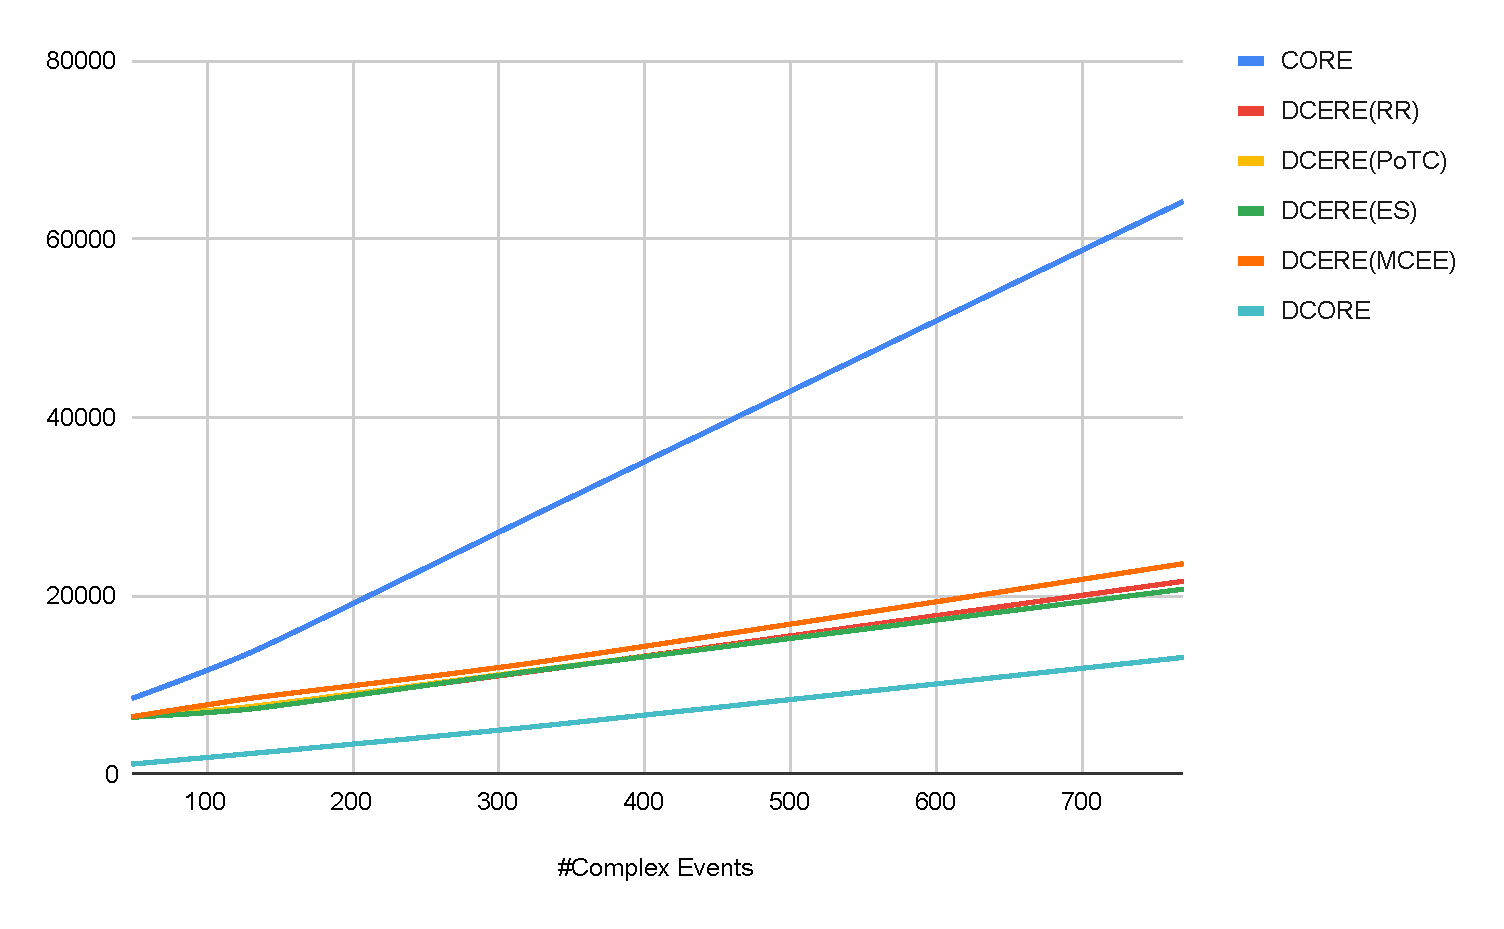
\includegraphics[scale=0.5]{experiment_1_chart_3}
  \caption{$Q_{1}$.}
  \label{fig:???}
\end{figure}

% A;B+;C
\begin{figure}[H]
  \centering
  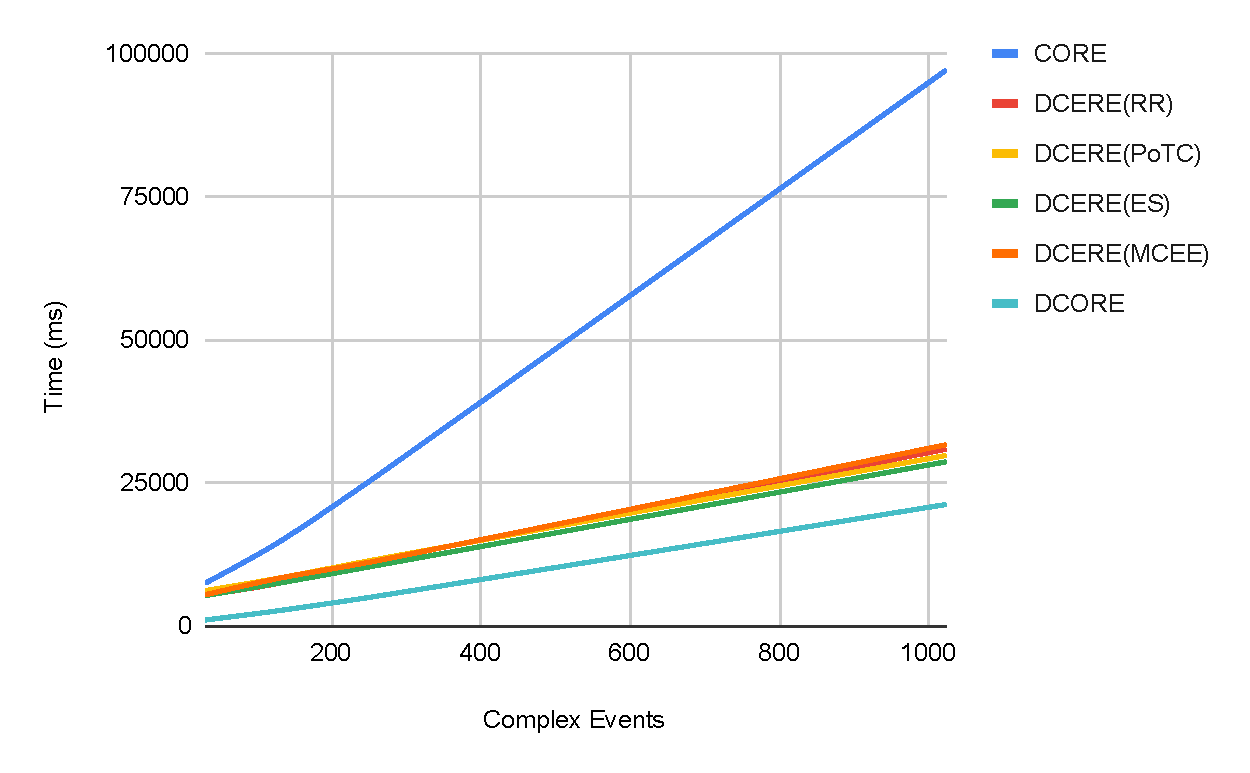
\includegraphics[scale=0.5]{experiment_1_chart_2}
  \caption{$Q_{2}$.}
  \label{fig:???}
\end{figure}

% A+;B+;C
\begin{figure}[H]
  \centering
  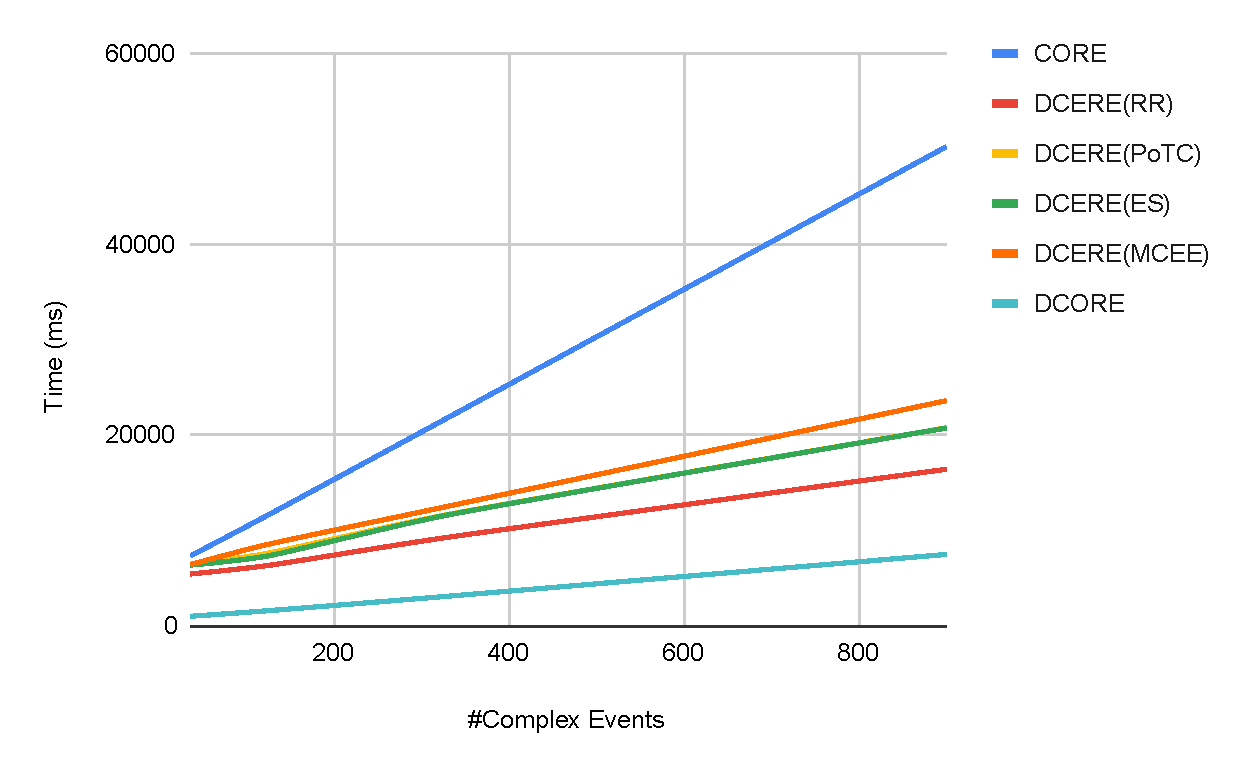
\includegraphics[scale=0.5]{experiment_1_chart_1}
  \caption{$Q_{3}$.}
  \label{fig:???}
\end{figure}


\textbf{Experimental results}.

\section{Experiments on the scalability of the framework}\label{sec:scalability}

% A;B;C
\begin{figure}[H]
  \centering
  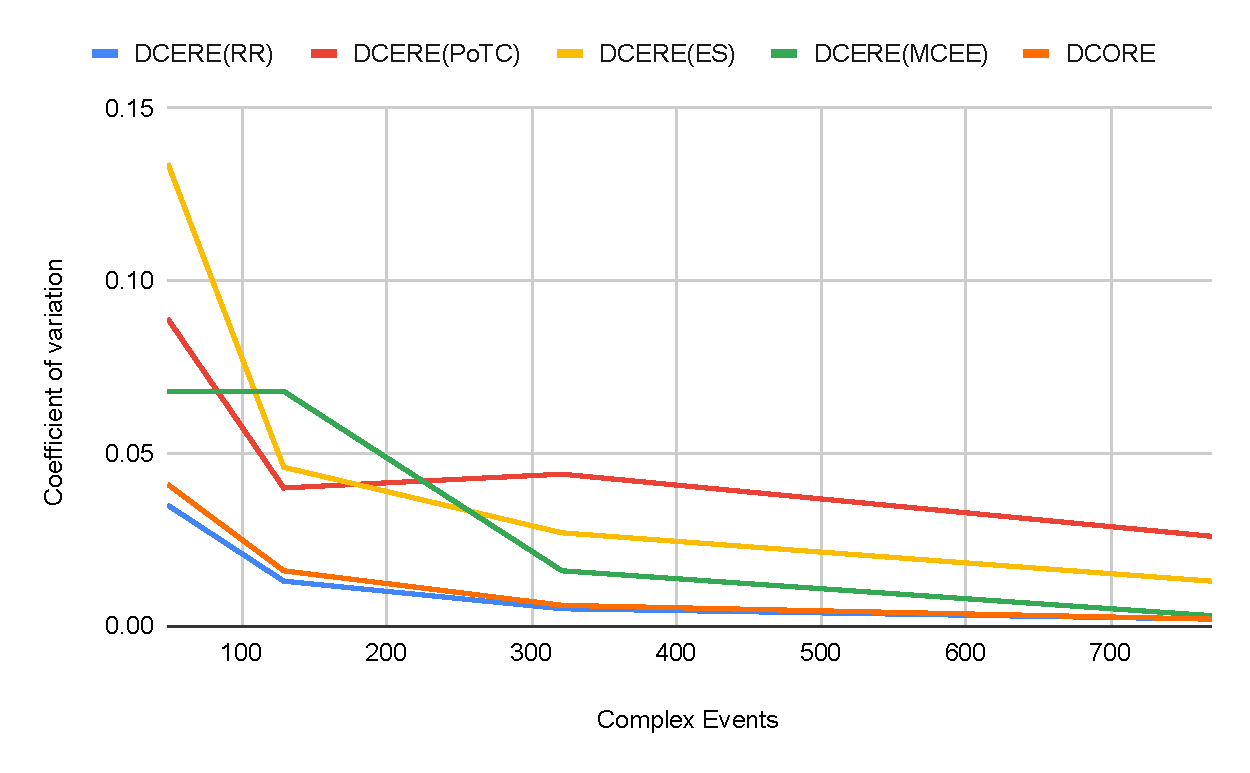
\includegraphics[scale=0.5]{experiment_2_chart_3}
  \caption{$Q_{1}$.}
  \label{fig:???}
\end{figure}

% A;B+;C
\begin{figure}[H]
  \centering
  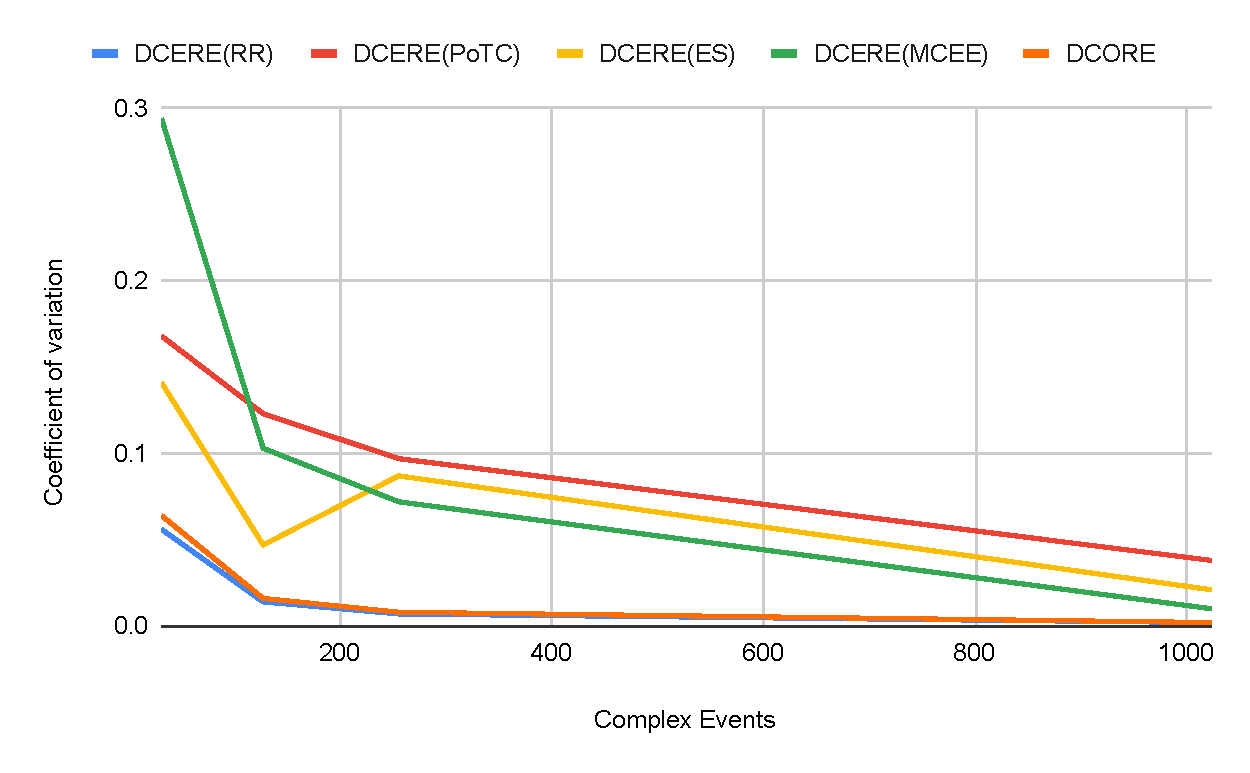
\includegraphics[scale=0.5]{experiment_2_chart_2}
  \caption{$Q_{2}$.}
  \label{fig:???}
\end{figure}

% A+;B+;C
\begin{figure}[H]
  \centering
  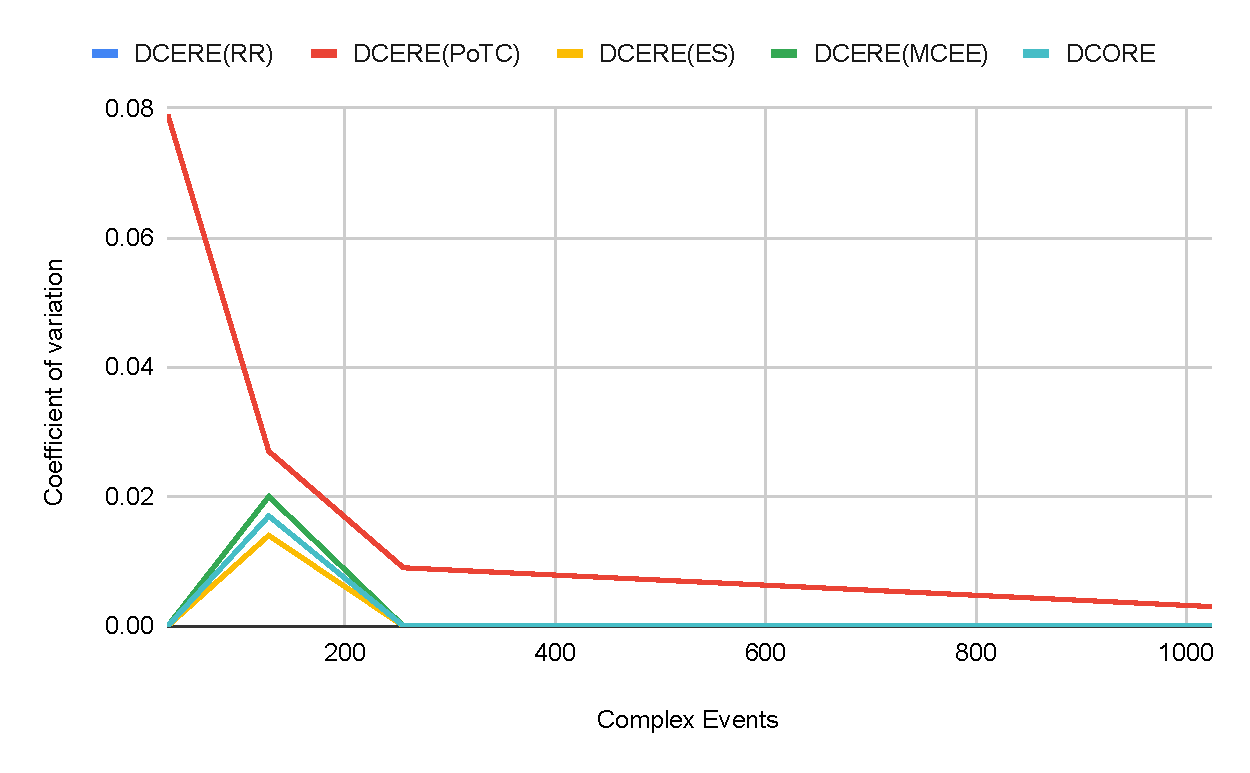
\includegraphics[scale=0.5]{experiment_2_chart_1}
  \caption{$Q_{3}$.}
  \label{fig:???}
\end{figure}



\begin{figure}[H]
  \centering
  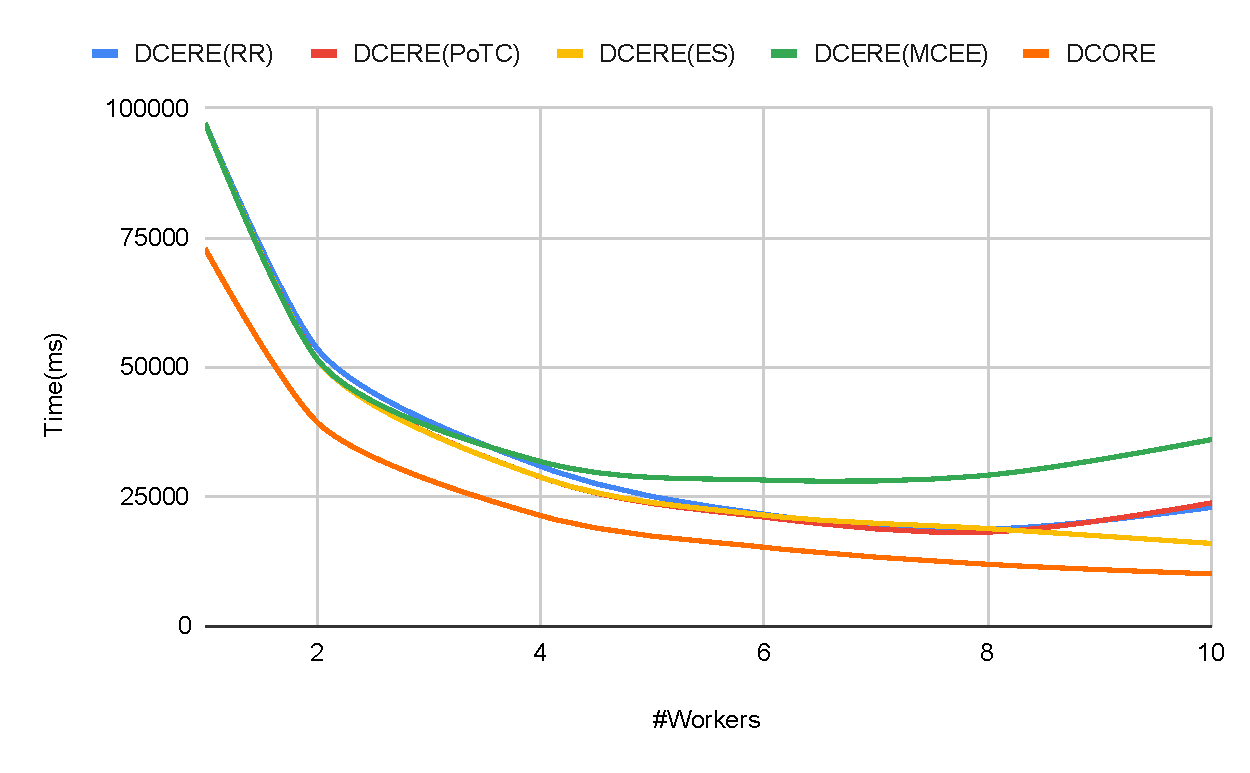
\includegraphics[scale=0.5]{experiment_3_chart_1}
  \caption{$Q_{2}$.}
  \label{fig:???}
\end{figure}

\begin{figure}[H]
  \centering
  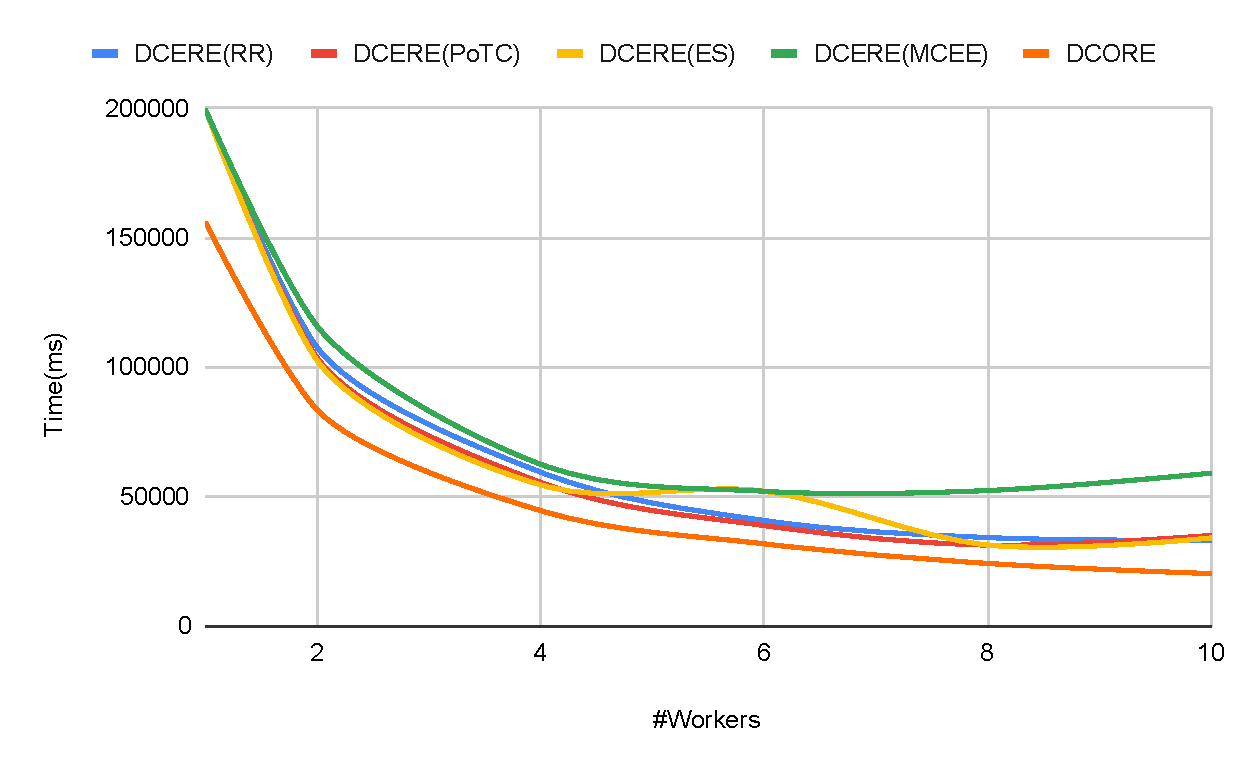
\includegraphics[scale=0.5]{experiment_3_chart_2}
  \caption{$Q_{2}$.}
  \label{fig:???}
\end{figure}

\textbf{Experimental results}.

\section{Experiments on the novel evaluation algorithm}\label{sec:new-algorithm}

% A;B;C
\begin{figure}[H]
  \centering
  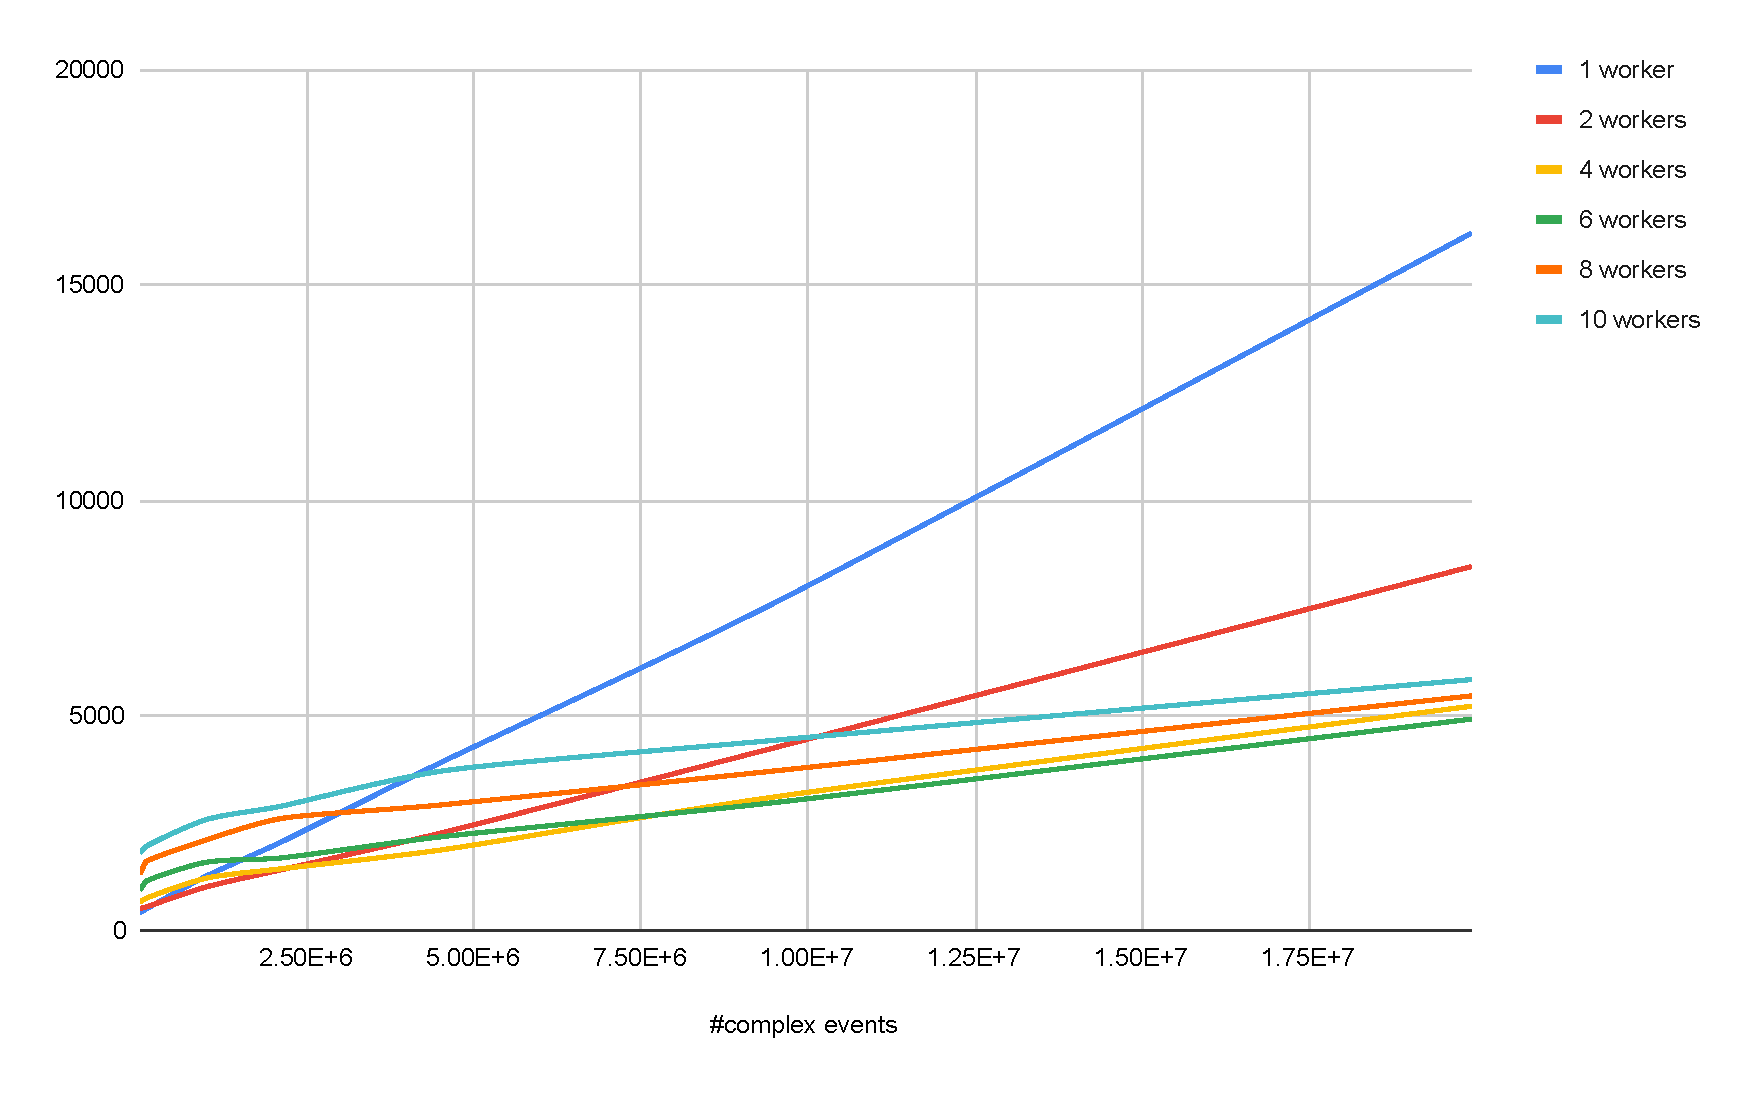
\includegraphics[scale=0.5]{experiment_4_chart_3}
  \caption{$Q_{1}$.}
  \label{fig:???}
\end{figure}
% A;B+;C
\begin{figure}[H]
  \centering
  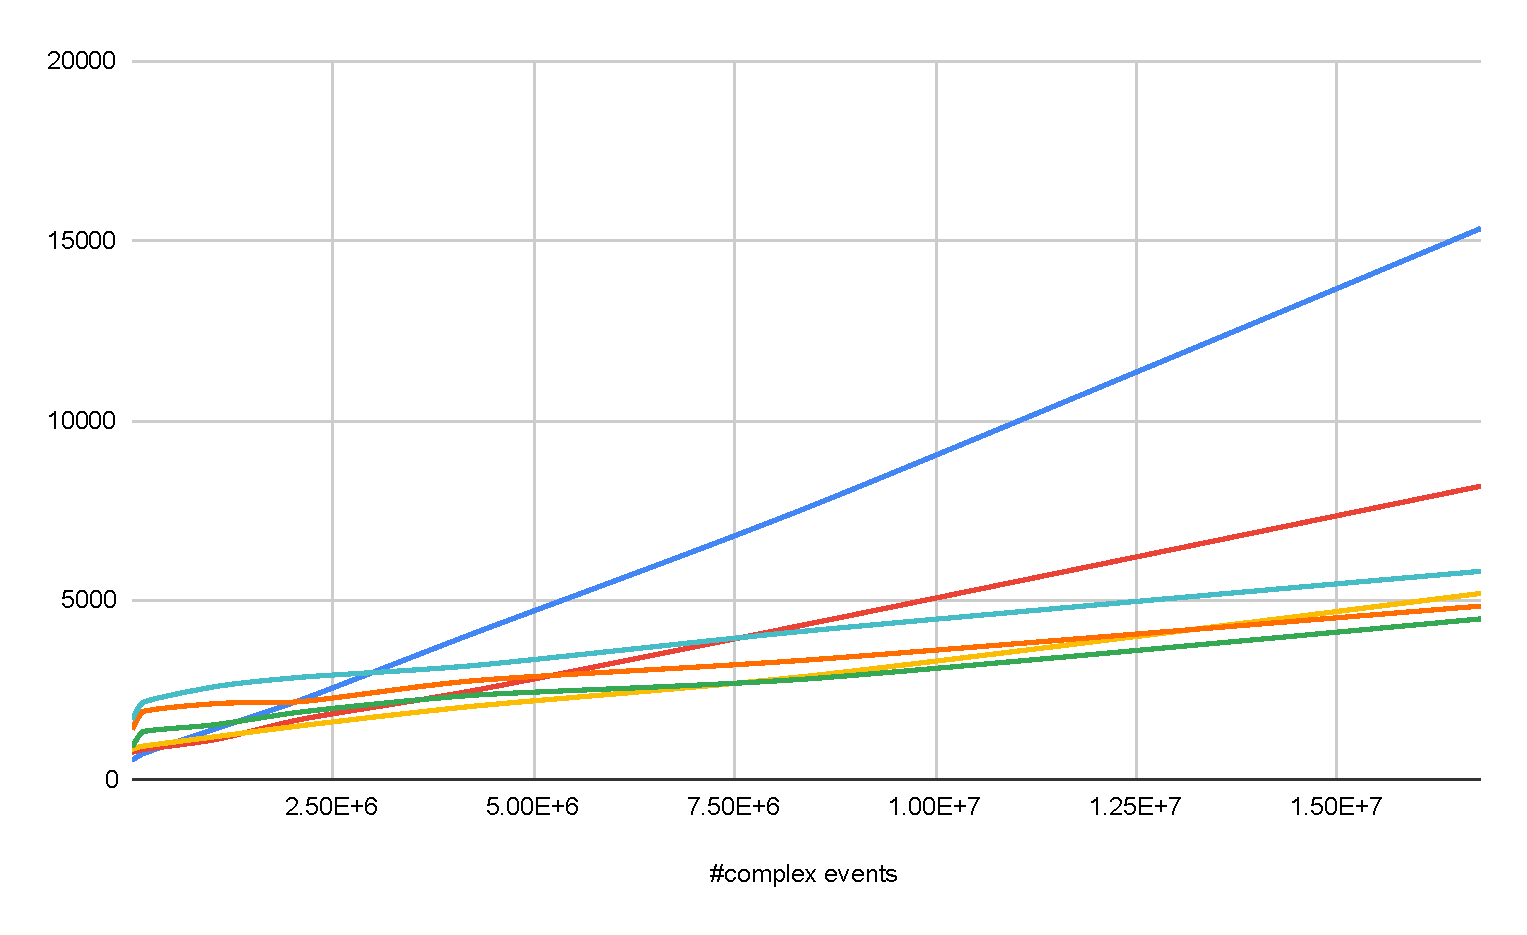
\includegraphics[scale=0.5]{experiment_4_chart_2}
  \caption{$Q_{2}$.}
  \label{fig:???}
\end{figure}
% A+;B+;C
\begin{figure}[H]
  \centering
  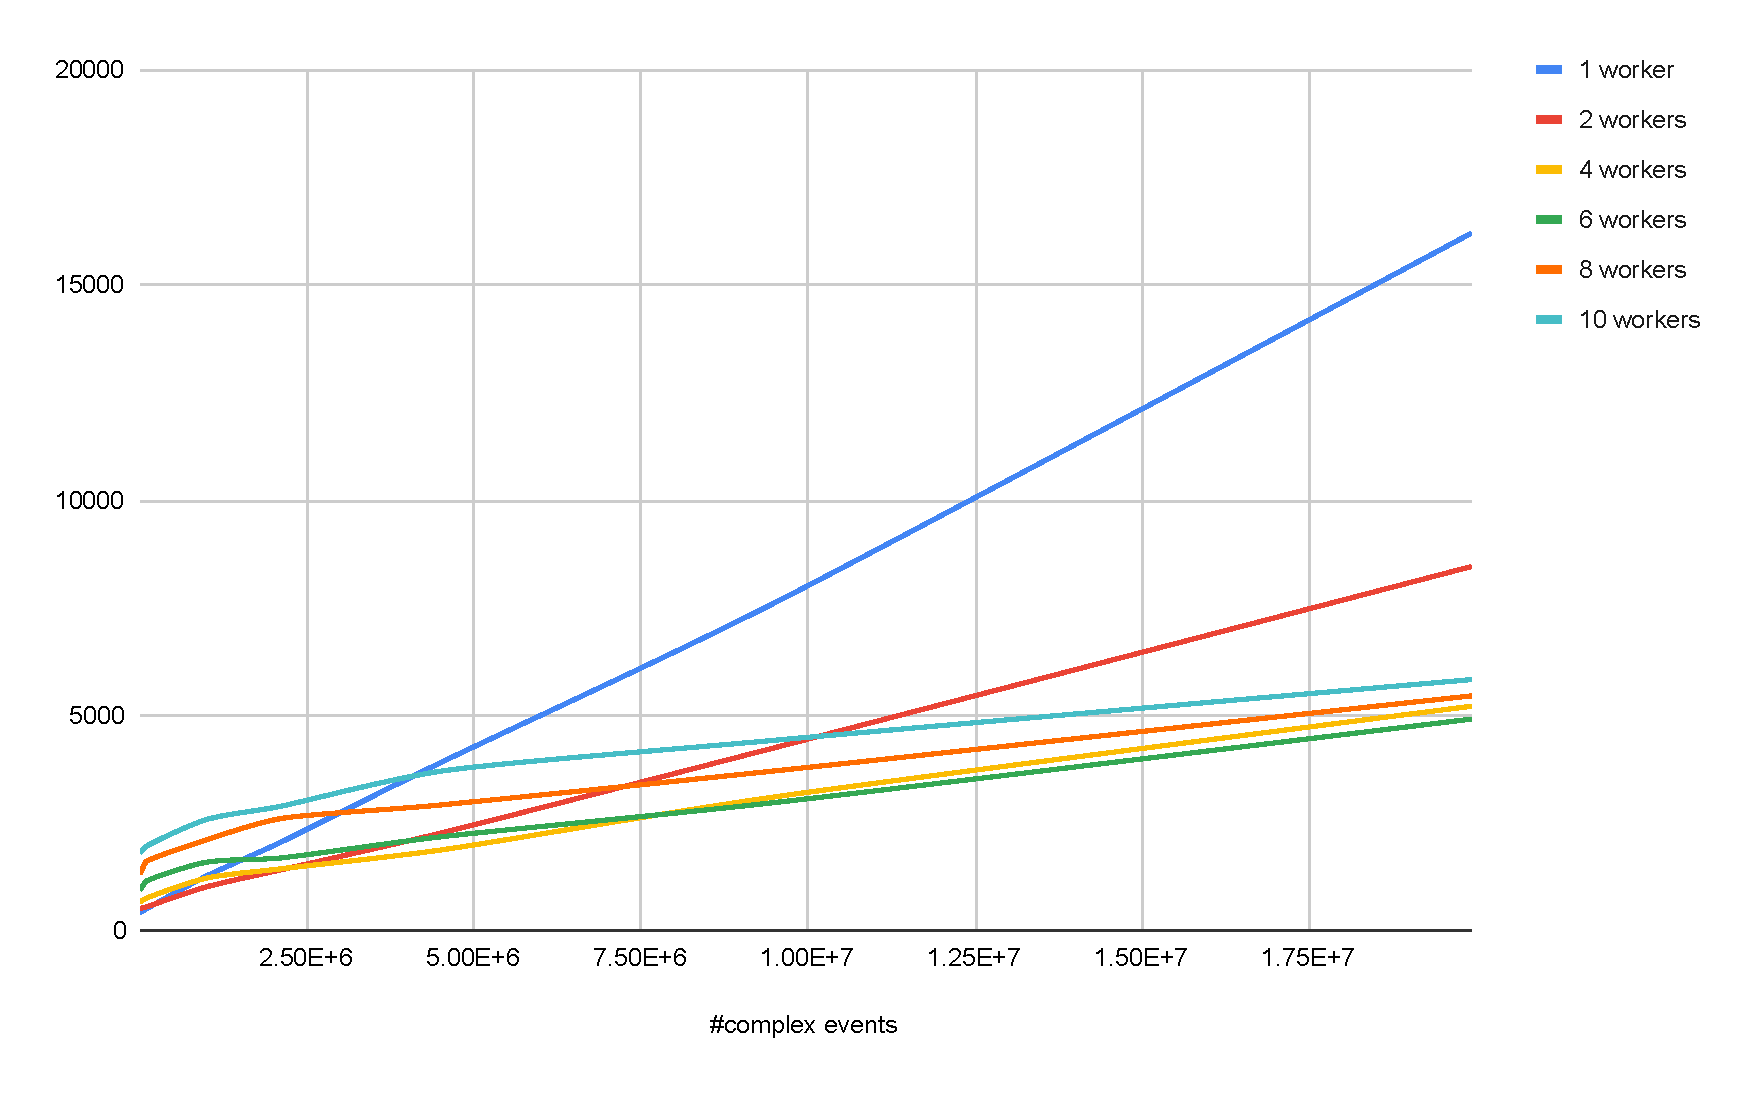
\includegraphics[scale=0.5]{experiment_4_chart_3}
  \caption{$Q_{3}$.}
  \label{fig:???}
\end{figure}


\begin{figure}[H]
  \centering
  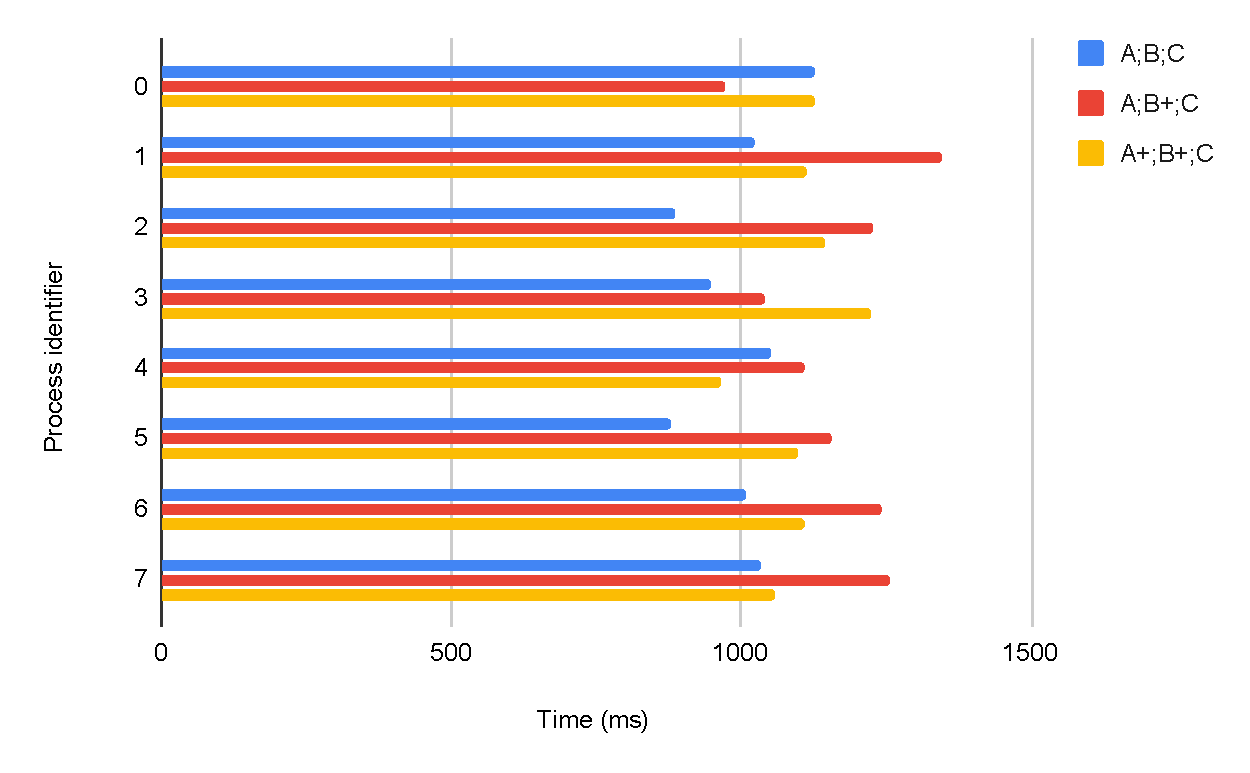
\includegraphics[scale=0.5]{experiment_5_chart_1}
  \caption{.}
  \label{fig:???}
\end{figure}

% 2 processors
\begin{figure}[H]
  \centering
  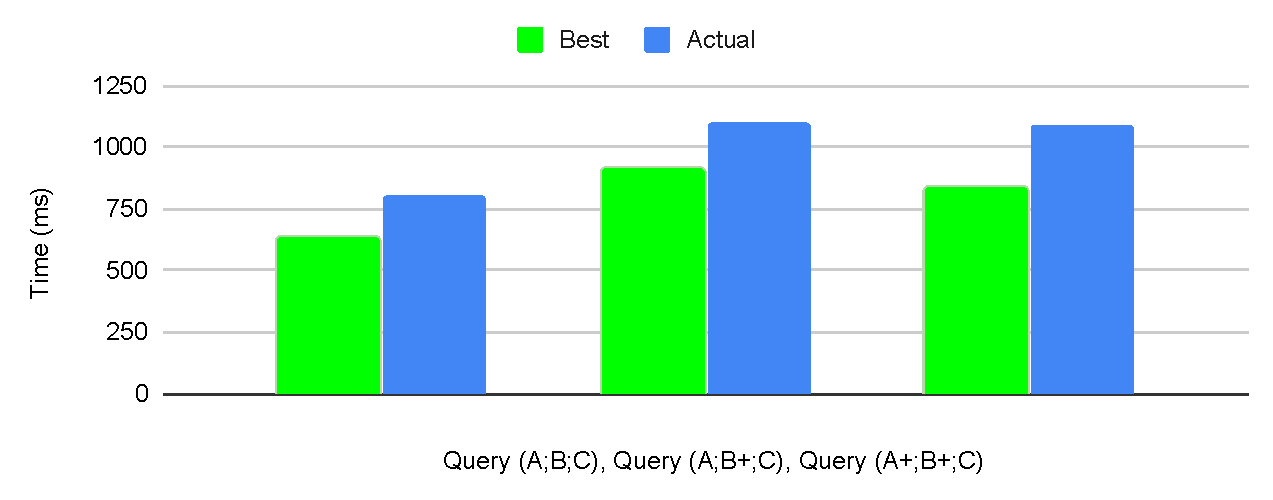
\includegraphics[scale=0.5]{experiment_5_chart_2}
  \caption{.}
  \label{fig:???}
\end{figure}

% 4 processors
\begin{figure}[H]
  \centering
  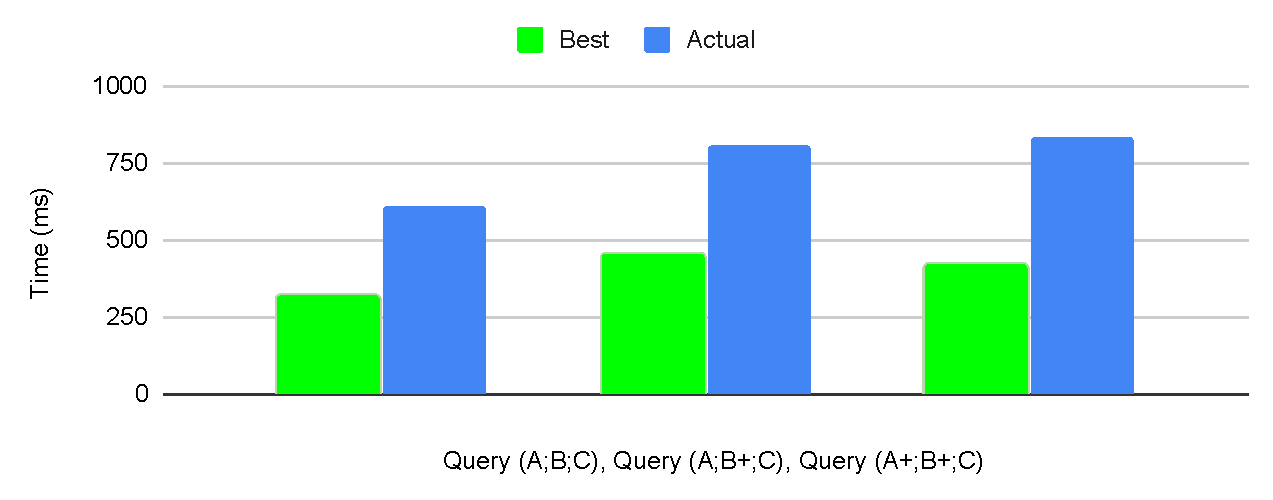
\includegraphics[scale=0.5]{experiment_5_chart_3}
  \caption{.}
  \label{fig:???}
\end{figure}

% 6 processors
\begin{figure}[H]
  \centering
  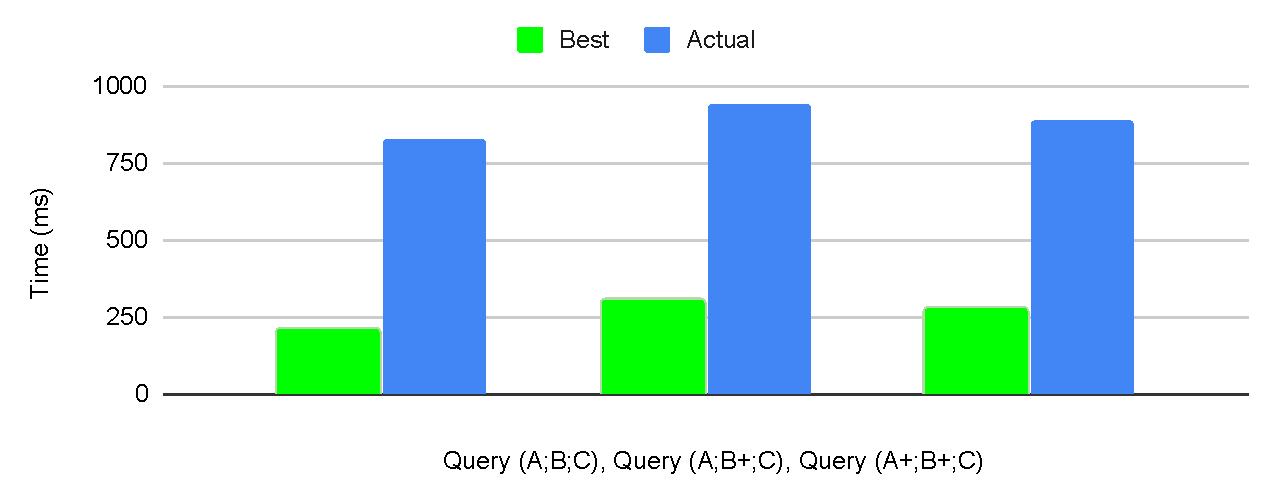
\includegraphics[scale=0.5]{experiment_5_chart_4}
  \caption{.}
  \label{fig:???}
\end{figure}

% 8 processors
\begin{figure}[H]
  \centering
  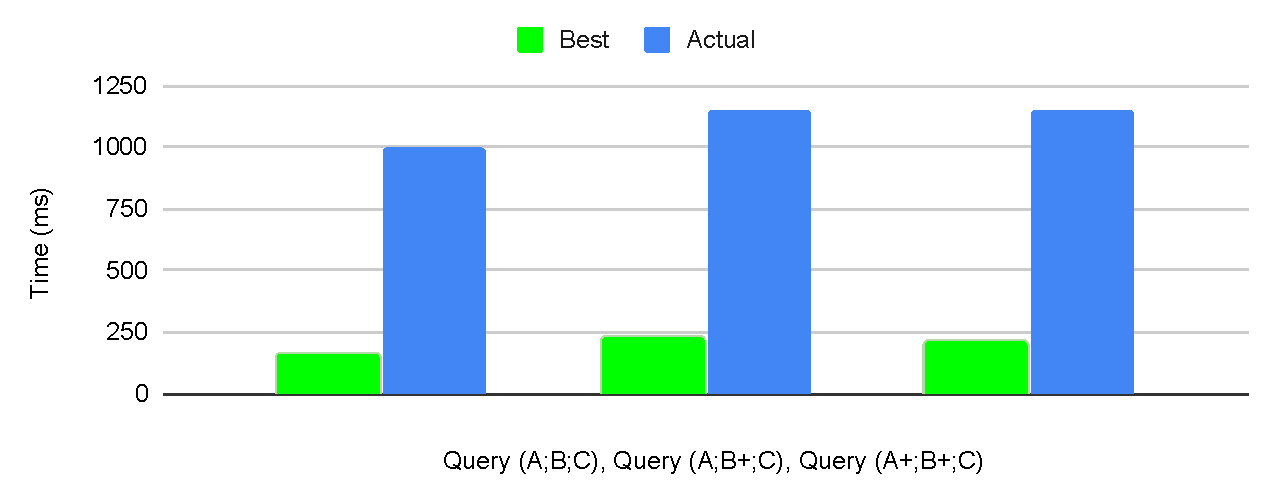
\includegraphics[scale=0.5]{experiment_5_chart_5}
  \caption{.}
  \label{fig:???}
\end{figure}

\textbf{Experimental results}.

\section{Chapter summary}

\chapter{Experimental evaluation}\label{chapter:experimental_evaluation}

\section{Implementation}
\label{sec:implementation}

\section{Reproducibility of the experiments}
\label{sec:reproducibility}



\section{Chapter summary}

\chapter{Conclusions and future work}\label{chapter:conclusion}

% \textbf{Note}. We implemented a rewrite and refine algorithm that only works for very specific queries. Implementing a generic rewrite and refine algorithm is outside of the scope of this thesis and it is left for future work.


\begin{appendices}
\chapter{}\label{appendix:A}

\section{Proof of Theorem~\ref{theorem:isomorphism}}\label{appendix:A:sec:1}

\begin{theorem}[${\llbracket \text{n} \rrbracket}^{\epsilon}_{\mathcal{E}}(j) \longleftrightarrow paths_{\ge j - \epsilon}(n)$]
  For every complex event within a time window of size $\epsilon$ there exists exactly one path that reaches a bottom node $b$ with $pos(b) \ge j - \epsilon$, and vice versa.
\end{theorem}

\begin{proof}
  Fix $j$, $\epsilon$, and $\mathcal{E}$. Let $n$ be a node in $\mathcal{E}$. The proof follows by the definition of ${\llbracket \text{n} \rrbracket}^{\epsilon}_{\mathcal{E}}(j)$, ${\llbracket \text{n} \rrbracket}_{\mathcal{E}}$, ${\llbracket \bar{p} \rrbracket}_{\mathcal{E}}$, and ${paths}_{\ge \tau}(n)$. Recall that

  \begin{itemize}
    \item ${\llbracket \text{n} \rrbracket}^{\epsilon}_{\mathcal{E}}(j) = \{ ([i,j], D) \ | \ (i,D) \in {\llbracket \text{n} \rrbracket}_{\mathcal{E}} \land j - i \le \epsilon \}$ encodes all open complex events represented by $n$ in $\mathcal{E}$ that, when closed with j, are within a time window of size $\epsilon$,
    \item ${\llbracket \text{n} \rrbracket}_{\mathcal{E}} = \bigcup\limits_{\bar{p};\\ start(\bar{p}) = n} {\llbracket \bar{p} \rrbracket}_{\mathcal{E}}$ encodes all open complex events ${\llbracket \bar{p} \rrbracket}_{\mathcal{E}}$ with $\bar{p}$ a full-path in $\mathcal{E}$ starting at $n$, and
    \item ${\llbracket \bar{p} \rrbracket}_{\mathcal{E}} = (i, D)$ where $\bar{p} = n_{1},n_{2}, \ldots, n_{k}$ be a \emph{full-path} in $\mathcal{E}$ such that $n_{k}$ is a bottom node, $i = pos(n_{k})$ is the label of the bottom node $n_{k}$, and $D$ is the set of labels of the other non-union nodes in $\bar{p}$.
  \end{itemize}

  First, we prove ${\llbracket \text{n} \rrbracket}^{\epsilon}_{\mathcal{E}}(j) \longmapsto paths_{\ge j - \epsilon}(n)$. Given a complex event $([i, j], D) \in {\llbracket \text{n} \rrbracket}^{\epsilon}_{\mathcal{E}}(j)$, there is an open complex event $(i, D) \in {\llbracket \text{n} \rrbracket}_{\mathcal{E}}$ that is represented as the full-path $\bar{p} = n_{1},n_{2}, \ldots, n_{k}$ in $\mathcal{E}$ such that $n_{k}$ is a bottom node and $i = pos(n_{k})$ is the label of the bottom node $n_{k}$. Notice, $n_{1} = n$ is the starting node, $j = pos(n_{1})$ is the label of the starting node $n_{1}$, and $j - i \le \epsilon$. By definition, $\bar{p} \in {paths}_{\ge \tau}(n)$.

  Secondly, we prove that $paths_{\ge j - \epsilon}(n) \longmapsto {\llbracket \text{n} \rrbracket}^{\epsilon}_{\mathcal{E}}(j)$. The proof follows by expanding the definition of ${paths}_{\ge \tau}(n)$ and following the steps of ${\llbracket \text{n} \rrbracket}^{\epsilon}_{\mathcal{E}}(j) \longmapsto paths_{\ge j - \epsilon}(n)$'s proof in reverse order.

  Finally, by ${\llbracket \text{n} \rrbracket}^{\epsilon}_{\mathcal{E}}(j) \longmapsto paths_{\ge j - \epsilon}(n)$ and $paths_{\ge j - \epsilon}(n) \longmapsto {\llbracket \text{n} \rrbracket}^{\epsilon}_{\mathcal{E}}(j)$ proofs, ${\llbracket \text{n} \rrbracket}^{\epsilon}_{\mathcal{E}}(j) \longleftrightarrow paths_{\ge j - \epsilon}(n)$ immediately holds.

\end{proof}

\section{Algorithms Chapter~\ref{chapter:distributed-cer}}\label{appendix:A:sec:2}

\subsection{Maximal Complex Event Enumeration}\label{appendix:A:sec:2:subsec:1}

\begin{algorithm}[H]
  \setstretch{0.9} % space between lines
  \DontPrintSemicolon
  \SetAlgoNoEnd % don't print end
  \SetAlgoNoLine % no vertical lines
  \LinesNumbered
  \SetKwProg{Procedure}{procedure}{}{}
  \SetKwFunction{MCEE}{\textsc{Mcee}}
  \SetKwFunction{Enumerate}{\textsc{Enumerate}}
  \SetKwFunction{Loop}{\textsc{Loop}}
  \SetKwFunction{Configurations}{\textsc{Configurations}}
  \SetKwFunction{Distribute}{\textsc{Distribute}}
  \SetKwFunction{Partition}{\textsc{Partition}}
  \SetKwFunction{Head}{head}
  \SetKwFunction{Type}{type}
  \SetKwFunction{Last}{last}
  \SetKwFunction{Enum}{enum}
  \SetKwFunction{GroupBy}{\textsc{GroupBy}}
  \SetKwFunction{Type}{type}
  \SetKwFunction{Event}{event}
  \SetKwFunction{Children}{children}
  \SetKwFunction{Add}{add}
  \SetKwFunction{Map}{\textsc{Map}}
  \SetKwFunction{NewNode}{new-node}

  \Procedure{\MCEE{$\mathcal{C}_{V}$, $\mathcal{P}$}}{
    $\mathcal{K} \leftarrow \emptyset$\;
    \For{$C_{V} \in \mathcal{C}_{V}$}{\label{algo:mcee:line:for:1}
        $\mathcal{K} \leftarrow \mathcal{K} \cup \Configurations{$C_{V}$}.\Map{$\lambda K \to \langle K, C_{V} \rangle$}$\;
    }
    $D \leftarrow $\GroupBy{$\mathcal{K}, \lambda \langle K, \_ \rangle \to K$}\;\label{algo:mcee:line:groupby}
    \Distribute{$\mathcal{P}, D$}\;
  }
  \;

  \Procedure{\Enumerate{$D$}}{
    \For{$\langle K, \mathcal{C_{V}} \rangle \in D$}{\label{algo:mcee:line:for:2}
      $T \leftarrow$ \text{\NewNode{}}\;\label{algo:mcee:line:new-node}
      \For{$C_{V} \in \mathcal{C}_{V}$}{\label{algo:mcee:line:for:3}
        $\mathcal{G} \leftarrow \Partition{$C_V$}$\;
        \Loop{$T, \mathcal{G}, \emptyset, \bot, K$}\;
        }
    }
  }
  \;

  \Procedure{\Loop{$n, \mathcal{G}, C_{V}, new, K$}}{
    \Switch{$\mathcal{G}$}{\label{algo:mcee:line:switch}
      \uCase{$\emptyset$}{\label{algo:mcee:line:case:1}
        \If{$new$}{\label{algo:mcee:line:if:1}
          \Return{$C_{V}$}
        }
      }
      \uCase{$G \cup \mathcal{G}$}{\label{algo:mcee:line:case:2}
        $k \leftarrow K(\Type{G})$\;
        $N \leftarrow \binom{G}{k}$\;
        \For{$i \in N$}{
          \eIf{$\exists n' \in \Children{n}. \ \ \Event{n'} = i$}{\label{algo:mcee:line:if:2}
            \Loop{$n', \mathcal{G}, C_{V} \cup i, new$}\;
          }{
            $n' \leftarrow $\NewNode{$i$}\;
            $\Add{\Children{n}, n'}$\;
            \Loop{$n', \mathcal{G}, C_{V} \cup i, \top, K$}\;
          }
        }
      }
    }
  }
\caption{Distributed enumeration of a set of maximal complex events $C_{V}$ over a set of workers $W$.}
\label{algo:mcee}
\end{algorithm}

Algorithm~\ref{algo:mcee} consist of two procedures: \textsc{Mcee} and \textsc{Enumerate}. The main procedure is \textsc{Mcee}, which is executed in the master actor, while \textsc{Enumerate} is executed on each slave actor. It receives as an input a set of \emph{maximal} complex events $\mathcal{C}_{V} := \{C^{1}_{V}, \ldots, C^{n}_{V}\}$ and a set of processing unit $\mathcal{P} := \{P_{1},\ldots, P_{n}\}$, and outputs all \emph{complex events} $C_{V}' \subseteq \mathcal{C}_{V}$ distributedly. The \code{for} (lines~3-4) compute the set of \emph{configurations} corresponding to each maximal complex event in $\mathcal{C}_{V}$ (see Algorithm~\ref{algo:configurations}) and pairs each configuration with its maximal complex event. A \emph{configuration} is a binary relation $T \times \mathbb{N}$ from data-tuples $t \in T$ to natural numbers. For example, given maximal complex event $C_{V} := \{T, T, H, H, H\}$, then $\code{Configurations}(C_{V}) = \{ \{T, 2\}, \{H, 3\}\}$.


\begin{algorithm}[H]
  \setstretch{0.9} % space between lines
  \DontPrintSemicolon
  \SetAlgoNoEnd % don't print end
  \SetAlgoNoLine % no vertical lines
  \LinesNumbered
  \SetKwProg{Procedure}{procedure}{}{}
  \SetKwFunction{Configurations}{\textsc{Configurations}}
  \SetKwFunction{Head}{head}
  \SetKwFunction{Type}{type}
  \SetKwFunction{Last}{last}
  \SetKwFunction{Enum}{enum}
  \SetKwFunction{OrdTypes}{ordered-types}
  \Procedure{\Configurations{$C_{V}$}}{
    \KwIn{A complex event $C_{V} = \{i, \ldots, j\}$ with $C_{V} \subseteq 2^{\mathbb{N}}$.}
    \KwOut{A set $\mathcal{K}$ of configurations $K := T \times \mathbb{N}$ where $K$ is the mapping from the event type $t \in T$ to the size of the group of consecutive events of type $t$ in the complex $C_{V}$.}
    $\mathcal{V} \leftarrow \emptyset$\;
    $i \cup C_{V}' \leftarrow \Head{$C_{V}$}$\;
    $A \leftarrow \{ i \}$\;
    $\Type{$A$} \leftarrow \Type{$i$}$\;
    \For{$j \in C_{V}'$}{
      \eIf{$\Type{$j$} = \Type{$A$}$}{
        $A \leftarrow A \cup j$\;
        \uIf{$\Last{$C_{V}$} = j$} {
          $\mathcal{V} \leftarrow \mathcal{V} \cup \Enum{$1, |A|$}$
        }
      }{
        $\mathcal{V} \leftarrow \mathcal{V} \cup \Enum{$1, |A|$}$\;
        $A \leftarrow \{ j \}$\;
        $\Type{$A$} \leftarrow \Type{$j$}$\;
      }
    }
    $\mathcal{W} \leftarrow \bigtimes\limits_{V \in \mathcal{V}} V$\;
    $T \leftarrow \OrdTypes{$C_{V}$}$\;
    $\mathcal{K} \leftarrow \emptyset$\;
    \ForEach{$W \in \mathcal{W}$}{
      $K \leftarrow \emptyset$\;
      \For{$i \leftarrow 1$ \KwTo $|W|$}{
        $K \leftarrow K \cup (T[i], W[i])$\;
      }
      $\mathcal{C} \leftarrow \mathcal{C} \cup C$\;
    }
    \Return{$\mathcal{C}$}
  }
\caption{Configuration of a complex event $C_{V}$.}
\label{algo:configurations}
\end{algorithm}


\textsc{GroupBy} of line~\ref{algo:mcee:line:groupby} groups the set of tuples $\mathcal{K} := \{\langle C_{V}, K \rangle, \ldots\}$ by their configuration resulting in the set of tuples $D := \{\langle K, \mathcal{C}_{V}\} \rangle, \ldots \}$, where $\mathcal{C}_{V} := \{C^{1}_{V}, \ldots, C^{m}_{V}\}$. Then, the set $D$ is distributed among the $|\mathcal{P}|$ processing units using a generic load-balancing algorithm \textsc{Distribute}. The choice of implementation does not affect the correctness of the algorithm.

The procedure \textsc{Enumerate} receives the set of tuples $D := \{\langle K, \mathcal{C}_{V}\} \rangle, \ldots \}$ and enumerates all complex events included in each $\mathcal{C}_{V}$ filtered by $K$. $K$ is a configuration and for each event type $T$, it returns the exact number of complex event of that type that must be present in the resulting complex events. This is what allows us to control the load-balancing of the process, by distributing the configurations assigned to each process. For each tuple $\langle K, \mathcal{C}_{V} \rangle$, lines~10-13 are executed. First, a new \emph{tree} root $T$ is created on line~\ref{algo:mcee:line:new-node}. This $n$-ary tree will be used through the algorithm to detect which complex events have been outputted before to avoid duplicates. Then, for each maximal complex event $C_{V} \in \mathcal{C}_{V}$, the procedure \textsc{Partition} is executed and the result is given to procedure \textsc{Enumerate'}.

The procedure \textsc{Partition} partitions the complex event $C_{V}$ in sets of consecutive positions of events of the same type. For example, \newline
\hspace*{60pt}$\textsc{Partition}(\{T, T, H, H, H\}) = \{\{T,T\}, \{H,H,H\}\}$

Procedure \textsc{Loop} receives as input a node $n$, a grouped complex event $\mathcal{G}$, a partial complex event $C_{V}$, a boolean $new$, and a configuration $K$ corresponding to complex event $C_{V}' \equiv \mathcal{G}$. On each iteration, \textsc{Loop} extends $C_{V}$ with the next group in $\mathcal{G}$ and the configuration $K$ associated to that group. The \code{switch} from line~\ref{algo:mcee:line:switch} is split in two cases. Case 1 (lines~17-19) corresponds to the base case when $\mathcal{G}$ is empty. If the complex event $C_{V}$ has not been outputted before (i.e., $new = \top$), then we output the complex event $C_{V}$ and stop, otherwise, we just stop. Case 2 (lines~20-29) corresponds to the inductive step when $\mathcal{G}$ has at least a group of events of the same type in the corresponding complex event $C_{V}'$. Notice, that $\mathcal{G}$ on each iteration is smaller, ergo the algorithm terminates. For each group of events of the same type $G$, $k \in \mathbb{N}$ is retrieved from the configuration $K$, which corresponds to the size assigned to that processing unit for the group $G$. Different processing units will have different sizes assigned to each group, resulting in disjoint complex events enumerated by each unit. The $k$-combination set $N := \binom{G}{k}$ is computed, where $N$ contains complex event positions. Then, for each $k$-combinations of events, lines~23-29 are executed. In both cases, $C_{V}$ is extended with positions $i \subseteq 2^{\mathbb{N}}$. If there exists a children node $n'$ in $n$ that contains events $i$, then we recursively call \textsc{Loop} with extended complex even $C_{V} \cup i$, but we do not update $new$ since an event such as $C_{V} \cup i$ has already been outputted before. Otherwise, we create a new node $n'$ with events $i$, extend our current node $n$ with $n'$, and, as before, we call \textsc{Loop}, but this time with argument $new = \top$ indicating that complex event $C_{V}$ has not been enumerated before.

\end{appendices}

\bibliographystyle{unsrtnat}
\bibliography{bibliography}

\end{document}
